\chapter{Introduction}

%--------------------------------------------------------
% Automata in general

Automata theory is a well-known field of study. Automata appear in our mundane lives every day. It is consequently important to study automata further and learn to cooperate with them too. Automata are also commonly used in mathematics and computation theory in general (e.g., in model checking \cite{DBLP:conf/cav/SiegelY20} or string solving and analysis \cite{DBLP:conf/popl/LinB16}). Of course, their uses in the field of logic are not to be forgotten (e.g., WS1S \cite{DBLP:conf/tacas/FiedorHJLV17, DBLP:journals/acta/FiedorHLV19}).

Our goal in this thesis is to explore possibilities of using various abstractions of automata languages in optimization of automata algorithms. We will study different approaches to abstraction of languages of states. We start with abstracting languages of states to sets of possible word lengths and to Parikh images, represented as semi-linear sets, and exploring options of using them to optimize the construction of synchronous product of automata by pjjruning pairs of states with incompatible abstractions. We then continue towards optimization of these techniques. We consider the use of mintermization and other approaches to further improve these methods.

Finite automata are easy to understand, but as soon as you start adding new states, transitions and additional accepting states, the finite automaton will get extensively larger and harder to work with.
Our focus is on several specific, often used operations over the finite automata, which are usually simple, but take lots of computational time and generate vast state space as a result. One of such operations over the automata is construction of their intersection. We use product construction and its emptiness test as a benchmarking operation in our experiments. Our suggested optimization methods are tested on the product construction algorithm, but are generally usable on many other typical automata algorithms. Consequently, even if our approaches to the optimization problems are introduced on product construction algorithms, our discoveries have wider impact and are in some form applicable on other automata operations, e.g., complement etc.

%--------------------------------------------------------
% Intersection

The intersection of two or more automata (the synchronous product construction) is often used in mathematics and logic. It is an extensively used operation where one follows the transitions in the original automata, trying to find such runs where all the original automata use the same transition symbols. Therefore, one can do the same run with the transition symbols for all of the finite automata at once in the product---assuming there is such a run---combining the original states from the individual runs to tuples called product states and adding them to the generated state space. For two automata, the classical algorithm starts with an initial state of both automata, make pairs from them and try to find transitions leading from these initial states in the original automata with the same symbol. Generate new pairs for found transitions, find their transitions, and so on. Every product state represents an intersection of languages of two corresponding states in the original automata.

Unfortunately, the synchronous product construction is expensive on computational time as one needs to generate a vast number of product states during the process. For two automata, the state space can increase quadratically, for more automata, the product state space increases exponentially according to the number of used automata and the number of their states. Furthermore, often there are large parts of the generated state space which cannot accept any words (non-terminating states), yet are still generated because of the corresponding transition symbols.

%--------------------------------------------------------
% Our optimization

We will try to optimize this process by reducing the number of generated product states and their transitions for both generating the synchronous product and deciding its emptiness test. We focus mainly on decision-making about the satisfiability problem-solving the emptiness of an intersection of two (eventually even multiple) finite automata. We consider length abstraction over the initial finite automata while trying to predict which product states cannot lead to any accepting states.

When the lengths of words recognized by the languages of the current states are not compatible with each other---the original languages of the corresponding states cannot accept a word of the same lengths---there is definitely no transition from this product state leading to accepting the same word in both original automata. We can omit such states from our generated product. Consequently, this removes the need to even consider their potential successor states, which are generated normally. By doing this, we trim the generated product state to only states whose corresponding original states languages can accept words of the same lengths. Even though there might still be states which do not lead to any accepting state in the final product, this simple optimization already trims a substantial parts of the normally generated synchronous product state space reasonably often.

%--------------------------------------------------------
% Length abstraction

Computing length abstraction over the languages of finite automata (and over individual states in the automata in particular) is accomplished using lasso automata (handle and loop automata)---deterministic finite automata with a unary alphabet (similar as in \cite{DBLP:conf/cav/AbdullaACHRRS14}). They consist of a \emph{handle} (a sequence of states from the initial state) and a single \emph{loop} (resolving the cycles in the original automaton) with a few accepting states along the way, hence the name of a handle and loop or lasso automaton. Create one by taking the initial automaton, consider all transition symbols as a single transition symbol and determinize this automaton.

What you get is an automaton accepting every length of any word recognized by the language of the initial automaton. Consequently, it is easy to compute semi-linear set (formulae\footnote{disjunction of linear equations}) for the allowed lengths of words, which can be effectively processed and compared using SMT solvers. We are computing these formulae for individual product states (precisely for the corresponding states in the original automata), checking their satisfiability and consequently construct only those product states for which the length test resolves as satisfiable.

%--------------------------------------------------------
% Parikh image

The second optimization approach we consider is the computation of Parikh images for potential product states. Computing Parikh image as a set of constraints for given product state to be included in the generated product. With Parikh images of such potential product states, we have additional information about the current state under consideration and can more precisely determine whether to include such state in the product state space. However, the Parikh image computation in itself is a demanding operation and the evaluation of satisfiability of mentioned constrains for every product state requires additional computation time.

In this case, it is necessary to decide whether the trade-off of unoptimized basic algorithm generating larger product state space requiring less computation time for reduced product state space generated by our optimized algorithms using Parikh images with additional computation time requirements is worth our attention. We say it is. For certain operations over the automata, the product state space size is crucial, considering we may need to work with the same product multiple times or simply need to execute a single operation on the product, reduced state space can spare extensive amounts of computation time further down the processing line. Furthermore, generating smaller state space using our Parikh image optimization can improve computation time for the sole product generation algorithm in case substantial parts of otherwise generated state space are pruned due to unsatisfiable constraints defined by Parikh image for any given product state in the process of generating the final product or even when the whole product is proved to be empty, which can be quickly determined by our optimization, whereas the classic unoptimized algorithms would proceed to generate useless fragments of suppositional product.

%--------------------------------------------------------
% Mintermization

Our another optimization uses mintermization as a different approach to abstracting state languages of initial automata. We compute minterms, which can be used instead of transition symbols while retaining all information about the automata to compute Parikh images and other optimization abstractions in less computation time.

%--------------------------------------------------------
% Experiments + Contributions

We have implemented these optimizations and experimented with several different automata, tried various combinations of them, generated their products and tried to solve their emptiness test, focusing mainly on the number of trimmed product states in the process. For certain types of automata of certain qualities, this optimization process works really well.

Our proposed algorithm cannot remove any product states leading to an actual accepting state. Therefore, it is impossible to accidentally trim product states leading to some accepting states and change the intersection language in the end. The language we get is the same as the one generated from the naive product construction algorithm. Consequently, is it completely secure to use our optimization with any kind of automata for any kind of uses.

The contribution of this work can be summarized as follows:
\begin{enumerate}
    \item heuristic trimming generated state space of finite automata synchronous product construction based on length abstraction, and
    \item implementation and experimental evaluation of said heuristic.
\end{enumerate}

%--------------------------------------------------------
%--------------------------------------------------------
%--------------------------------------------------------
%--------------------------------------------------------

\chapter{Preliminaries}
Let us clarify a few definitions and terms often used throughout this paper. The following definitions are mostly adapted from \cite{Esparza} or \cite{Sipser}.

\emph{Alphabet} is a finite, non-empty set denoted by $\Sigma$. Elements of an alphabet are called \emph{symbols} or \emph{letters}. A finite, possibly empty sequence of symbols over an alphabet is a \emph{word} $w$ from the set of all words $\Sigma^*$ over an alphabet $\Sigma$.

\begin{definition}[\textbf{Deterministic finite automaton}] \hfill \newline
    A deterministic finite automaton (DFA) is a 5-tuple $A = (Q, \Sigma, \delta, I, F)$, where:
    \begin{itemize}
        \item Q is a non-empty \textbf{set of states},
        \item $\Sigma$ is an \textbf{input alphabet},
        \item $\delta$ is a \textbf{transition function}: $Q \times \Sigma \rightarrow{} Q$,
        \item $I \in Q$ is the \textbf{initial state}, and
        \item $F \subseteq Q$ is a \textbf{set of final states}.
    \end{itemize}
\end{definition}

A \emph{run} of $A$ on input $a_0a_1a_2...a_{n-1}$ is a sequence $q_0 \xrightarrow{a_0} q_1 \xrightarrow{a_1} q_2 \xrightarrow{a_3} ... \xrightarrow{a_{n-1}} q_n$, such that $q_i \in Q$ for $0 \leq i \leq n$ and $\delta(q_i, a_i) = q_{i+1}$ for $0 \leq i \leq n - 1$. A run is \emph{accepting} if $q_n \in F$. The automaton A accepts a word $w \in \Sigma^*$ if it has an accepting run on input $w$. A \emph{language} recognized by finite automaton A is a set $L(A) = \{w \in \Sigma^* | w \text{ is accepted by } A\}$. A single transition from transition function $\delta$ is denoted as $q \xrightarrow{a} q'$ if $q' \in \delta(q, a)$ and means \textit{one can get from state $q$ to state $q'$ with a transition symbol $a$}. For every state, DFA has at most one transition for a given symbol.

\begin{definition}[\textbf{Non-deterministic finite automaton}]
    A non-deterministic finite automaton (NFA) is a 5-tuple $A = (Q, \Sigma, \delta, I, F)$, where $Q$, $\Sigma$ and $F$ are as for DFA and:
    \begin{itemize}
        \item $\delta$ is a \textbf{transition relation}: $\delta: Q \times \Sigma_{\epsilon} \rightarrow{} P(Q)$, where $\Sigma_{\epsilon} = \Sigma \cup \epsilon$ and $P(Q) = \{R | R \subseteq Q\}$ is a set of subsets of $Q$, and
        \item $I = \{q | q \in Q\}$ is a non-empty \textbf{set of initial states}.
    \end{itemize}
\end{definition}

Consequently, DFA has exactly one run on a given word from initial state to one of the accepting states (or nonterminating states in case the word is not accepted by the automaton at all). For every state and its transition symbol $P(Q) \in \delta(q, a)$ is a singleton. For example, $\delta(q_1, a) = \{ q_1, q_2 \}$.

Two finite automata $A$ and $B$ are said to be \emph{equivalent} when both accept the same language: $L(A) = L(B)$.

For every NFA $A$ exists a corresponding DFA $B$. \emph{Determinization} is a process of converting such NFA to DFA.

\begin{definition}[\textbf{Powerset (\textbf{subset}) construction}]
    The powerset construction is a method for creating a corresponding deterministic finite automaton from its equivalent non-deterministic finite automaton. Produces finite automaton $A'$, where $Q' = 2^Q$, $F' = \{S \in Q' | S \cap F \neq \emptyset\}$, $I' = I$ and for $S \in Q': \delta'(S, a) = \bigcup_{s \in S} \delta(s, a)$.
\end{definition}

\begin{definition}[\textbf{Product construction}]
Operations \\ on automata $A_1$ and $A_2$ yield a result~-- a product $A$ as a 5-tuple deterministic finite automaton $A = (Q, \Sigma, \delta, I, F)$.

Given two NFAs $A_1 = (Q_1, \Sigma, \delta_1, I_1, F_1)$ and \\ $A_2 = (Q_2, \Sigma, \delta_2, I_2, F_2)$ over the same alphabet $\Sigma$, we can define:
\begin{itemize}
    \item a set of states $Q = Q_1 \times Q_2$,
    \item a transition relation $\delta: Q \times \Sigma \rightarrow{} P(Q)$,
    \item a set of initial states $I = I_1 \times I_2$, and
    \item a set of accepting states $F = F_1 \times F_2$.
\end{itemize}
\end{definition}

The transition relation is described as $\delta = \\ ([q_1, q_2], a) = \delta_1(q_1, a) \times \delta_2(q_2, a)$. For pairs of states $q_1$ and $q_2$ from $A_1$ and $A_2$, respectively, and a common transition symbol $a$ of transitions $q'_1 \in \delta_1(q_1, a)$ and $q'_2 \in \delta_2(q_2,a)$, we denote a single product transition as $[q_1, q_2] \xrightarrow{a} [q'_1, q'_2]$, where $[q'_1, q'_2] \in \delta([q_1, q_2], a)$ for the corresponding states $[q_1, q_2]$ and $[q'_1, q'_2]$ in $A$ are called product states.

Focusing mainly on \emph{intersection} of automata, the product construction tells that
$$ L(A) = L(A_1) \cap L(A_2) \text{.} $$

To solve the \emph{emptiness test}, we test
$$ L(A) = \emptyset \text{.}$$

\begin{algorithm}
\caption{Classic product construction}\label{productConstructionAlg}
\SetKwData{Left}{left}\SetKwData{This}{this}\SetKwData{Up}{up}
\SetKwFunction{Union}{Union}\SetKwFunction{FindCompress}{FindCompress}
\SetKwInOut{Input}{Input}\SetKwInOut{Output}{Output}
\DontPrintSemicolon
\Input{ NFA $A_1 = (Q_1, \Sigma, \delta_1, I_1, F_1)$, \\ NFA $A_2 = (Q_2, \Sigma, \delta_2, I_2, F_2)$}
\Output{ NFA $(A_1 \cap A_2) = (Q, \Sigma, \delta, I, F)$ with $L(A_1 \cap A_2) = L(A_1) \cap L(A_2)$}
\BlankLine
$Q, \delta, F \gets \emptyset$ \\
$I \gets I_1 \times I_2$ \\
$W \gets  I$

\While{$W \neq \emptyset$}{
    \textbf{pick} $[q_1, q_2]$ \textbf{from} $W$ \\
    \textbf{add} $[q_1, q_2]$ \textbf{to} $Q$ \\
    \If{$q_1 \in F_1$ and $q_2 \in F_2$} {
        \textbf{add} $[q_1, q_2]$ \textbf{to} $F$
    }
    \ForAll{$a \in \Sigma$}{
        \ForAll{$q'_1 \in \delta_1(q_1, a), q'_2 \in \delta_2(q_2, a)$}{
            \If{$[q'_1, q'_2] \notin Q$}{\textbf{add} $[q'_1, q'_2]$ \textbf{to} $W$}
            \textbf{add} $[q'_1, q'_2] \textbf{ to } \delta([q_1, q_2], a)$
        }
    }
}
\end{algorithm}\DecMargin{1em}

\section{Parikh Image Computation} %TODO
\begin{definition}[\textbf{Parikh Image}]
\end{definition}

%--------------------------------------------------------
%--------------------------------------------------------
%--------------------------------------------------------
%--------------------------------------------------------

\chapter{State Language Optimizations}

In this chapter, we will intruduce several optimizations of state language. We aim to optimize operations on finite automata such as product construction, complement computation, minimalization or determinization and inclusion test. Furthermore, we want to introduce state language optimizations which work for different automata structures. E.g., operations on transducers, operations with alternating automata such as its emptiness or conversion of alternating automaton to its NFA representation, conversion of finite automata to flat automata, etc.

Not only the classic operations are generally useful, but both transducers and alternating automata are operations often used, beside others, for example, in verification. Our optimization methods therefore have the ability to improve substantially important processes used throughout multitude of places and fields of study as well as in praxis.

We perform experiments with our optimization methods mostly on product construction of two NFAs and our optimization method algorithms are consequently introduced on these algorithms, improving the naive product construction algorithm to generate optimized products. Nevertheless, our optimization techniques are to be used in various fields of automata theory and allow us to optimize other, more complex problems. We chose product construction as our benchmarking operation on automata for its straightforwardness allowing us to see clearly pruning capabilities of our proposed optimization methods, even though the naive product construction algorithm complexity can be at most \emph{only} quadratic and is not that expensive in terms of computational time. Our optimization methods are applicable for more complex operations for exponential constructions (determinization, minimization, emptiness of alternating automaton, \ldots) and worse.

%--------------------------------------------------------
%--------------------------------------------------------

\section{State Language Optimization with Length Abstraction}

Our task is to try to minimize the number of generated states when trying to resolve the product construction of automata intersection and test its emptiness. One possible solution is looking for lengths of words accepted by both automata---testing whether both automata recognize words of the same lengths. Afterwards, we check the original transition symbols for generating new product states\footnote{So we do not get non-empty intersection results when there is no word both original automata actually accept and only their lengths correspond.}. Consequently, we can resolve the emptiness test of some intersections very quickly and optionally optimize the product construction, when we need to generate the whole product.

We will explain our chosen approach to the problem of optimizing product construction and deciding its emptiness test using length abstraction, but first some rudimentary knowledge on length abstraction is needed.

%--------------------------------------------------------
%--------------------------------------------------------
\subsection{Length Abstraction Represented by Lasso Automata} \label{sec:length_abstraction}

Our chosen approach to the problem of optimizing product construction and deciding its emptiness test includes using length abstraction over the finite automata to try to guess which product states do not lead to any final states and consequently can be omitted, and the following states do not need to be generated at all.

Length abstraction generalizes the language recognized by the initial automaton by considering only the possible lengths of words accepted by the automaton. It is an over-approximation of the language accepted by the original automaton. For us, this means if a word is not accepted by the length abstraction automaton, it cannot be accepted by the initial automaton either.

The length abstraction automaton is represented by a so-called lasso automaton. Let us demonstrate creation of the lasso automaton on the following simple non-deterministic finite automaton $A_1$, which we will continue to use in this paper to depict our optimization algorithm.

$$ A_1 = (\{q_0, q_1, q_2, q_3, q_4, q_5\}, \{0, 1\}, \delta_1, \{q_0\}, \{q_4\}) $$

Transition relation $\delta_1$ is depicted in Figure~\ref{fig:NFA_A1_orig}.

\begin{figure}[ht]
	\centering
	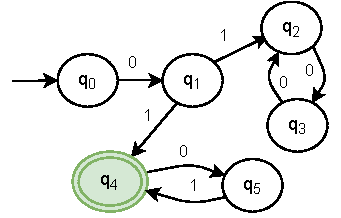
\includegraphics[width=0.7\linewidth]{diagrams-Original A.pdf}
	\caption{Non-deterministic finite automaton $A_1$}
	\label{fig:NFA_A1_orig}
\end{figure}

NFA $A_1$ is a non-deterministic finite automaton (see state $q_1$) and accepts more than one input symbol. Due to the fact that we work only with recognized word lengths, we can substitute automaton alphabet with unary alphabet of single input symbol (we have chosen $*$ for demonstration purposes)\footnote{Even though we do not actually need any particular input symbol, we use \emph{*} here as an example to depict the process. In general, all we need to know is that there is a transition between two states, the transition symbols are not significant for our optimization algorithm.}. Then, we can compute lasso automaton for our original automaton $A_1$ with unary alphabet, which is its deterministic equivalent.

$$\Sigma = \{0, 1\} \longrightarrow \Sigma' = \{*\} $$

\begin{figure}[ht]
	\centering
	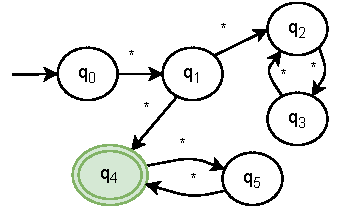
\includegraphics[width=0.7\linewidth]{diagrams-Original A Star.pdf}
	\caption{Non-deterministic finite automaton $A_1$ with unified transition symbols}
	\label{fig:NFA_A1_star}
\end{figure}

We start the determinization process on our updated automaton. For the final lasso automaton $A'_1$ for the original automaton $A_1$, see Figure~\ref{fig:HaL_A1}. This automaton now accepts any words of lengths of words recognized by the original automaton. We will use these lengths in the process of constructing the product.\footnote{You can notice this lasso automaton looks different to what is depicted in Section~\ref{sec:length_abstraction}. It is caused by our optimization with generating only one single lasso automaton per original automaton. The generated automaton is valid and the fact there are actually two separate automata with one even being inaccessible does not raise any issue for us. The reason for this behaviour will be further explained in Section~\ref{sec:singleHaL}.}

 \begin{figure}[ht]
	\centering
	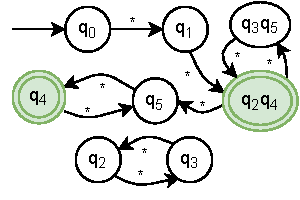
\includegraphics[width=0.7\linewidth]{diagrams-Final Handle and Loop Automaton A.pdf}
	\caption{Lasso automaton $A'_1$ for the original NFA $A_1$}
	\label{fig:HaL_A1}
\end{figure}



%--------------------------------------------------------
%--------------------------------------------------------
\subsection{Single Lasso Automaton for Each Original Automaton}\label{sec:singleHaL}

When we are constructing a product, we do not want to regenerate the lasso  automaton $L$ for each new product state $q$. This is inefficient. Therefore, our algorithm generates $L$ only once---state by state---checking every time, whether the new state $l$ is not already present in a set of states $Q_L$ of $L$.

Due to the nature of lasso automata, the successive product states generate the lasso automata very similar to $L$. We just need to append new states to $Q_L$. As a result, we will work with only two lasso automata (possibly with multiple loops and/or multiple handles)---one for both automata whose intersection is computed.

If $l \notin Q_L$, we add $l$ to $Q_L$ and continue with the following states $l'$ until we either create an entirely new loop in $L$ or generate $l' \in Q_L$. If $l \in Q_L$, we can stop generating $l'$ for $q$ as $\forall l' ( l' \in Q_L)$.

%--------------------------------------------------------
%--------------------------------------------------------
\section{Product Construction with Length Abstraction Optimization}

The core of the product construction algorithm remains unchanged, but there are a few differences. The Algorithm~\ref{productConstructionLengthAbstrAlg} shows how we alternate the original product construction algorithm to optimize it and resolve emptiness test for each \emph{branch} of the potential product automaton.

\begin{algorithm}
\caption{Product construction with length abstraction}\label{productConstructionLengthAbstrAlg}
\SetKwInOut{Input}{Input}\SetKwInOut{Output}{Output}
\DontPrintSemicolon
\Input{ NFA $A_1 = (Q_1, \Sigma, \delta_1, I_1, F_1)$, \\ NFA $A_2 = (Q_2, \Sigma, \delta_2, I_2, F_2)$}
\Output{ NFA $(A_1 \cap A_2) = (Q, \Sigma, \delta, I, F)$ with $L(A_1 \cap A_2) = L(A_1) \cap L(A_2)$}
\BlankLine
$Q, \delta, F \gets \emptyset$ \;
$I \gets I_1 \times I_2$ \;
$W \gets I$ \;\label{work_set}
$sat \gets False$ \;\label{sat}
$solved \gets \emptyset$ \;\label{solved}
\While{$W \neq \emptyset$}{
    \textbf{picklast} $[q_1, q_2]$ \textbf{from} $W$\label{picklast} \;
    \textbf{add} $[q_1, q_2]$ \textbf{to} $solved$ \;
    $sat \gets \mathbf{satisfiable(}[q_1, q_2]\mathbf{)}$\label{satisfiable} \;
    \If{$sat$}{\label{AlgSolveForSat}\label{satTrue}
        \textbf{add} $[q_1, q_2]$ \textbf{to} $Q$ \;
        \If{$q_1 \in F_1$ \textbf{and} $q_2 \in F_2$} {
        \textbf{add} $[q_1, q_2]$ \textbf{to} $F$ \;
        }\label{AlgAddToFinalState}
        \ForAll{$a \in \Sigma$}{
            \ForAll{$q'_1 \in \delta_1(q_1, a), q'_2 \in \delta_2(q_2, a)$}{
                \If{$[q'_1, q'_2] \notin solved$ \textbf{and} $[q'_1, q'_2] \notin W$}{
                    \textbf{add} $[q'_1, q'_2]$ \textbf{to} $W$ \;
                }
                \textbf{add} $[q'_1, q'_2] \textbf{ to } \delta([q_1, q_2], a)$ \;
            }
        }
    }
}
\end{algorithm}\DecMargin{1em}

We will call $W$ from line \ref{work_set} a work set. It stores the potential product states prepared for testing for satisfiability and other processing, which we pick from $W$ one by one\footnote{In spite of the fact that more approaches are valid, we strongly recommend picking the last added product state from the work set $W$ (see line \ref{picklast})---using Depth-first Search for a graph algorithm---as this allows us to quickly advance through the automaton and get to any final state faster---in case we just want to know whether automata have a non-empty intersection, this change will get us the answer most of the time in less steps. It works even better with implemented satisfiable state skipping optimization, explained in Section~\ref{sec:skipping states}.}.

The optimization process starts when a product state $q$ is picked from $W$. Instead of immediately generating new successive product states, we test $q$ for satisfiability of length constraints of recognized words from $q$. On line \ref{satisfiable}, we check for satisfiability of formulae generated from $q$. If the process shows formulae are satisfiable, i.e., there will be an accepting run using $q$ (see line \ref{satTrue}), we add $q$ to $Q$, possibly to $F$ and generate its successive product states $q'$.

% TODO: Update paragraphs and include implementation of satisfiable().
\begin{algorithm}
\caption{Check satisfiability using length abstraction algorithm with SMT solver}\label{checkLengthAbstractionSatisfiabilitySMTAlgorithm}
\SetKwInput{Input}{Input}
\SetKwInput{Output}{Output}
\SetKw{Return}{return}
\SetKwFunction{FIsLengthAbstractionSatisfiable}{isLengthAbstractionSatisfiable}%
\SetKwProg{Fn}{Function}{:}{}

\DontPrintSemicolon
\BlankLine

\Fn{\FIsLengthAbstractionSatisfiable{formulaeForFA1, formulaeForFA2}}{
    \KwData{
    Input length formulae of potential product state we are solving the satisfiability for (for all possible accept states combinations).\\
    formulaeForFA1: Formulae for the first finite automaton, \\
    formulaeForFA2: Formulae for the second finite automaton.
    }
    \KwResult{bool: \emph{True} if satisfiable, \emph{False} otherwise.}

    $smtAdd(VariableForFormulaForFA1 \geq 0, VariableForFormulaForFA2 \geq 0)$ \;

    \For{$formulaForFA1 \in formulaeForFA1$}{
        \For{$formulaForFA2 \in formulaeForFA2$}{
            $smtPush()$ \; % TODO Remove push and pop and replace the smtAdd with something like smtSetClauses.
            $smtAdd(formulaForFA1.handle + formulaForFA1.lasso * VariableForFormulaForFA1 = formulaForFA2.handle + formulaForFA2.lasso * VariableForFormulaForFA2)$ \;
            $sat \gets \textbf{smtCheck}()$ \;
            \If{$sat$ \textbf{ or } $sat = unknown$}{
                \Return $True$ \;
            }
            $smtPop()$ \;
        }
    }

    \Return $False$ \;
}

\end{algorithm}\DecMargin{1em}

The formulae are generated using lasso automata for both original automata. For every state, we get one or more formulae in the form $\varphi: \exists k( |w| = a + b \cdot k)$, where $|w|$ is a length of a recognized word, $a$ is the length of a handle to a certain accepting state, and $b$ is the length of a loop to return to this particular accepting state going through the loop. $k$ is the number of cycles through the loop states until a word ends in an accepting state. When multiple depicted formulae are present (because there are more accepting states in the lasso automaton), we append these formulae with \emph{logical or} ($\lor$), then compare these with the formulae from the other lasso automaton for the other initial finite automaton using SMT solver.

To better demonstrate our solution, the second automaton we will be working with is a finite automaton $A_2$ from Figure~\ref{fig:NFA_A2_orig}.

$$ A_2 = (\{s_0, s_1, s_2, s_3\}, \{0, 1\}, \delta_2, \{s_0\}, \{s_3\}) $$

Transition relation $\delta_2$ is depicted in Figure~\ref{fig:NFA_A2_orig}.

\begin{figure}[ht]
    \centering
	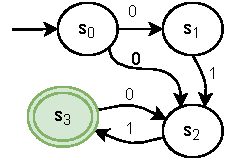
\includegraphics[width=0.7\linewidth]{diagrams-Original B.pdf}
	\caption{Non-deterministic finite automaton $A_2$}
	\label{fig:NFA_A2_orig}
\end{figure}

In Figure~\ref{fig:HaL_A2}, there is its lasso automaton $A'_2$, which we will be using together with the lasso automaton shown earlier in Figure~\ref{fig:HaL_A1} for computation of recognized word lengths.

\begin{figure}[ht]
    \centering
	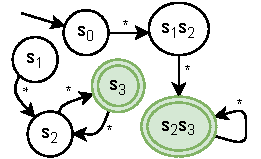
\includegraphics[width=0.7\linewidth]{diagrams-Final Handle and Loop Automaton B.pdf}
	\caption{Lasso automaton $A'_2$ for the original NFA $A_2$}
	\label{fig:HaL_A2}
\end{figure}

For automaton $A_1$ for the initial state (we start computing lengths as if the state $q_0$ is the initial state) from $A'_1$, we get quantifier-free formula $\varphi$\footnote{This formula consists of two independent formulae describing there are more possible lengths for accepted words from the same initial state (leading to two independent accepting states in the automaton).}. For automaton $A_2$ for the initial state from the lasso automaton $A'_2$, we get formula $\psi$\footnote{We are using variable $l$ here instead of $k$ to emphasize variables from different formulae are not dependent on each other---they correspond to various accepting states.}.
\begin{align*}
    &\varphi: \exists k(|w| = 2 \lor |w| = 4 + 2 \cdot k) \\
    &\psi: \exists l(|w| = 2 + 1 \cdot l)
\end{align*}

When we compare $\varphi$ and $\psi$, we get:
$$ \exists k \exists l (2 \lor 4 + 2 \cdot k = 2 + 1 \cdot l) $$

We try to find values of $k$ and $l$ such that some of the expressions on the left and on the right side of the equation are equal. We pass this equation to SMT solver to solve its satisfiability. Returns \emph{sat} when satisfiable ($sat$ is set to \emph{True}) and \emph{unsat} when unsatisfiable ($sat$ is set to \emph{False}). If \emph{unsat} is returned, we can stop generating this \emph{branch} of a NFA as we know for sure there cannot be a word which is accepted by both of these automata, when there is even no word fulfilling the length requirements. In this case, we have successfully reduced the generated state space by omitting this particular tested product state and any further product states, which would be later normally generated from these product states and its successors (assuming the transition symbols correspond).

\begin{figure}[ht]
	\centering
	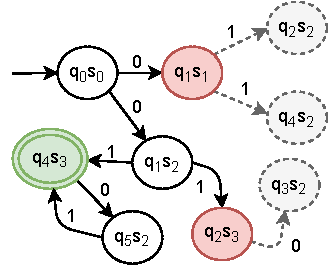
\includegraphics[width=0.7\linewidth]{diagrams-WIP Product.pdf}
	\caption{Constructed product automaton with depiction of our optimization.}
	\label{fig:product_WIP}
\end{figure}

In Figure~\ref{fig:product_WIP}, we can see the product of $A_1$ and $A_2$ being constructed using our optimization. Red states represent tested states that are resolved as unsatisfiable for computed length formulae and therefore the algorithm omits any successive product states---dashed states (such as $q_4s_2$ or $q_3s_2$), which are generated in the basic naive product construction algorithm. The green state is satisfiable and also represents accepting states in both automata. Here, we have found a possible solution accepted by both original automata. If we desire to resolve only the product emptiness test, we can stop the execution of the algorithm here as we have found one accepting state---automata have non-empty intersection.

\begin{figure}[ht]
	\centering
	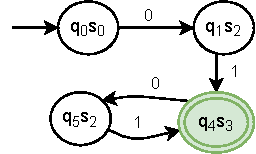
\includegraphics[width=0.7\linewidth]{diagrams-Final Product.pdf}
	\caption{Final product generated by our product construction algorithm optimizing its process by omitting unnecessary states on the way.}
	\label{fig:product_final}
\end{figure}

As you can notice in Figure~\ref{fig:product_final}, the product generated by our algorithm has only 4 product states in comparison to 9 product states generated by the classic algorithm.

When we get the result of formulae being unsatisfiable, we do not need to construct any following states and check their products for satisfiability and therefore, we are able to determine whether such \textit{branches} of automata have an empty intersection and we do not need to consider them in the product construction. The emptiness test is successfully accomplished, and we determined that for this \emph{branch} there cannot exist any word accepted by both automata and consequently by their intersection. When we get unsatisfiable result for every branch of the automaton (i.e., no \emph{branch} can lead to any accepting state) even if by inspecting transition symbols it looks like there could be a non-empty intersection, we can say that such input automata have an empty intersection and product construction will be very quick in that case---this is where our optimization dominates.

A note of caution. It is important to understand that we are working only with possible word lengths and therefore when we test the emptiness of intersection of automata, we can resolve only such intersections that words lengths are not accepted by both automata. When the test shows there could be some words of certain length accepted by both automata and for that reason by their intersection too (the result of the length abstraction satisfiability check is \emph{sat}), we cannot be sure there truly are any words accepted by both automata with their intersection non-empty, because there may be words of the suggested length, but it may be a different word for each automaton (which differ from one another in the containing symbols or their position in the word). For resolving such cases, we have to proceed with the classic algorithm steps to produce product states according to their original transition symbols, not only by comparing the possible words lengths. With certainty, we can omit only the cases where the length abstraction satisfiability check returns \emph{unsat}.

%--------------------------------------------------------
%--------------------------------------------------------

\subsection{Optimization with Skipping Satisfiable States} \label{sec:skipping states}

When we take a new product state $q$ from work set $W$ and check for satisfiability with formulae for $q$ being satisfiable, it is time to add to $W$ all of the possible successive product states $q'$. When $q$ generates only a single $q'$, we can say with certainty formulae for $q'$ are satisfiable too as there is only a single branch in the automaton leading from $q$ to an~accepting state (through $q'$). Product state $q'$ is \emph{skippable}, if exists a satisfiable $q$ whose only successor is $q'$. We add $q'$ to $W$ with the information of being skippable. If $q'$ is already in~$W$, we append the information to $q'$ in $W$.

We skip checking for the satisfiability when we pick $q'$ from $W$. We can immediately check for final states and generate the successive product states. This optimization saves us generating the length abstraction formulae for $q'$ and testing the formulae in the SMT solver for their satisfiability and even possibly reducing the number of states generated for both our lasso automata.

If our original automata have long lines (with non-splitting branches), this will prove extremely useful, because only a few proper iterations with formulae computing and executing SMT solver will be executed. In Algorithm~\ref{productConstructionLengthAbstrAlgSkip} is depicted the application of skipping satisfiable states. The line~\ref{satisfiable} from Algorithm~\ref{productConstructionLengthAbstrAlg} is substituted with the contents of Algorithm~\ref{productConstructionLengthAbstrAlgSkip}.


%{ \LinesNotNumbered
\begin{algorithm}
\SetKwFunction{FSkippable}{skippable}
\SetKwFunction{FSatisfiable}{satisfiable}
    \caption{Substitution of line~\ref{satisfiable} in Algorithm~\ref{productConstructionLengthAbstrAlg} with skipping satisfiable states.} \label{productConstructionLengthAbstrAlgSkip}
    \DontPrintSemicolon
    \eIf{$\textbf{not } \FSkippable{$[q_1, q_2]$}$}{
        $sat \gets \FSatisfiable{$[q_1, q_2]$}$ \;
    }{\label{AlgIsSkippable} % else
        $sat \gets True$ \;
    }
\end{algorithm}\DecMargin{1em}
%}

The only change is a test for every checked product state $q$, which decides whether $q$ can be skipped, if it cannot give us any information which we do not have yet. You can see that we proceed with SMT solver satisfiability check only for $q$ which are generated from the product states with multiple transitions generating $q$ and at least one more product state (in general at least two new potential product states). If only one $q$ is generated, we skip the satisfiability check for $q$ and continue to generating its successive states immediately.

\begin{figure}[ht]
	\centering
	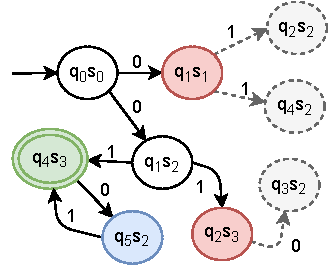
\includegraphics[width=0.7\linewidth]{diagrams-skip WIP Product .pdf}
	\caption{Constructed product automaton with depiction of skipping states optimization}
	\label{fig:wip_skip_product}
\end{figure}

You can notice there is one skippable state in the former example, which had to be evaluated and tested for satisfiability earlier. The blue state in Figure~\ref{fig:wip_skip_product} is such a skippable state. In our case for state $q_5s_2$, when only one new state is generated from state $q_4s_3$ while this state is resolved as satisfiable, newly generated product state has to be satisfiable as well, because the check for $q_4s_3$ already considered the state $q_5s_2$ as its only way to any accepting state resolving in \emph{sat} check for $q_4s_3$ actually.

When we have a series of such states, though, we can highly optimize generating the whole branch with only one initial check for satisfiability. In real world examples, there are often automata with long branches splitting into multiple branches only occasionally. We will check for satisfiability for all of the initial states of each new branch and then either omit the entire branch (if \emph{unsat} is returned) or skip checking satisfiability in the entire branch (if \emph{sat} is returned).


\subsection{Resolving Length Abstraction Satisfiability without SMT Solver}

% TODO: Comment on SMT solver removal for length abstraction.

\begin{algorithm}
\caption{Check satisfiability using length abstraction algorithm without SMT solver}\label{checkLengthAbstractionSatisfiabilitySMTFreeAlgorithm}
\SetKw{Return}{return}
\SetKwFunction{FIsLengthAbstractionSatisfiable}{isLengthAbstractionSatisfiable}
\SetKwFunction{FSolveForOneHandleLonger}{solveForOneHandleLonger}
\SetKwFunction{FGetGCD}{getGCD}
\SetKwProg{Fn}{Function}{:}{}

\DontPrintSemicolon
\Fn{\FIsLengthAbstractionSatisfiable{formulaeForFA1, formulaeForFA2}}{
    \KwData{
    Input length formulae of potential product state we are solving the satisfiability for (for all possible accept states combinations).\\
    formulaeForFA1: Formulae for the first finite automaton, \\
    formulaeForFA2: Formulae for the second finite automaton.
    }
    \KwResult{bool: \emph{True} if satisfiable, \emph{False} otherwise.}

    % The function code itself.
    \For{$formulaForFA1 \in formulaeForFA1$}{
        \For{$formulaForFA2 \in formulaeForFA2$}{
            \uIf{$formulaForFA1.handle = formulaForFA2.handle$}{
                \Return $True$ \;
            } \uElseIf{$formulaForFA1.handle > formulaForFA2.handle$}{
                $sat \gets \FSolveForOneHandleLonger{formulaForFA1, formulaForFA2}$ \;
                \If{$sat$}{
                    \Return $True$ \;
                }
            } \uElse{
                $sat \gets \FSolveForOneHandleLonger{formulaForFA2, formulaForFA1}$ \;
                \If{$sat$}{
                    \Return $True$ \;
                }
            }
        }
    }

    \Return $False$ \;
}
\BlankLine
\Fn{\FSolveForOneHandleLonger{formulaForFA1, formulaForFA2}}{
    \KwData{
    Input length formulae of potential product state we are solving the satisfiability for (for concrete accept states combination).\\
    formulaForFA1: Formula for the first finite automaton, \\
    formulaForFA2: Formula for the second finite automaton.
    }
    \KwResult{bool: \emph{True} if satisfiable, \emph{False} otherwise.}

    % The function code itself.
    $formulaForFA1.handle \gets formulaForFA1.handle - formulaForFA2.handle$ \;
    $formulaForFA2.handle \gets 0$ \;

    \uIf{$formulaForFA1.lasso = 0 \textbf{ and } formulaForFA2.lasso = 0$}{
        \Return $False$ \;
    } \uElseIf{$formulaForFA2.handle = 0$}{
        \Return $False$ \;
    } \uElseIf{$formulaForFA1.lasso = 0$}{
        $currentIteration \gets 0$ \;
        \While{$currentIteration \leq formulaForFA1.handle$}{
            \eIf{$currentIteration = formulaForFA1.handle$}{
                \Return $True$ \;
            }{
                $currentIteration \gets currentIteration + formulaForFA2.lasso$ \;
            }
            \Return $False$ \;
        }
    } \uElse{
        $gcd \gets \FGetGCD{formulaForFA1.lasso, formulaForFA2.lasso}$ \;
        \eIf{$gcd = 1$}{
            \Return $True$ \;
        }{
            $y \gets - formulaForFA1.handle$ \;
            \While{$y < gcd$}{
                $y \gets y + formulaForFA1.lasso$ \;
            }
            \eIf{$y \textbf{ mod } gcd = 0$}{
                \Return $True$ \;
            } {
                \Return $False$ \;
            }
        }
    }
    \Return $False$ \;
}
\end{algorithm}\DecMargin{1em}


%--------------------------------------------------------
%--------------------------------------------------------
%--------------------------------------------------------
%--------------------------------------------------------
\section{Product Construction Optimization with Parikh Image Computation}

This section presents a product construction optimization using Parikh images of finite automata. Parikh image optimization provides more information about the finite automata the product is computed for than simple length abstraction, which allows us to more precisely determine whether the generated product has non-empty intersection. However, the Parikh image computation itself consumes a considerate amount of computational time for some of the more extensive finite automata. The question is, whether the added computation time compensates for more precise product generation with higher product states pruning capabilities.

In this section, we will introduce an algorithm for Parikh image computation used for computing Parikh image of each potential product state to decide the satisfiability of Parikh image constraints for this particular product state. If the constraints are proved to be satisfiable, the considered product state is added to the generated product, otherwise, the potential product state is omitted and and no additional potential product states accessible from the omitted product state in one step are added to the queue for testing for their satisfiability.

%TODO
\subsection{Parikh Image} \label{sec:parikhImage}

We derive our Parikh image construction from the Parikh's theorem described in~\ref{ParikhsTheoremSimpleAndDirectConstruction}, creating a semilinear Parikh image formulae for the given regular language as a set of Parikh images for each word in the language. However, our usage of Parikh image of some regular language (and therefore of the corresponding finite automaton recognizing such regular language) is restricted to determine the satisfiability of Parikh image formulae. That is, Parikh image constrains which we use in SMT solver to represent the abstraction of the current potential product state language.

Our Parikh image formulae consist of the following constraints (clauses), in conjunctive normal form. For each potential product state, there exists exactly one our formula of Parikh image describing its regular language. We ask the SMT solver whether the Parikh image constraints for corresponding states in the original automata (one state per automaton) are compatible with each other. This ensures that we construct only those product states which satisfy the Parikh image constraints, otherwise we deem such potential product states redundant and such states can be pruned.

Given an NFA $A = (Q, \Sigma, \Delta, q_0, F)$, Parikh image constraints representing clauses in the classic Parikh image formula are constructed as follows:
\begin{enumerate}
    \item \label{clauses:u_original} Foremost, we define a variable $u_{q}$ for each transition $t \in \Delta$. We assign values to $u_{q}$ as follows:
    \begin{itemize}
        \item $u_{q} = 1$ for the initial state $q_0$,
        \item $u_{q} \in \{ 0, -1 \}$ for each state $q \in F$ and
        \item $u_{q} = 0$ for every other state $q \in Q \ ( \{ q_{o} \} \cup F )$.
    \end{itemize}

    \item \label{clauses:y_original} Second, we define a variable $y_{t}$ for each transition $t \in \Delta$ such that $y_{t} \geq 0$.

    \item \label{clauses:uy_original} We can now present an equation introducing a connection between $u_{q}$ and $y_{t}$ for each automaton state $q \in Q$ as follows:
    $$ u_q + \sum_{t \in \Delta_q^+} y_t - \sum_{t \in \Delta_q^-} y_t = 0.$$
    where $\Delta_q^+$ is a set of ingoing transitions $ \Delta_q^+ = \{ (q',a,q) \in \Delta \}$ and $\Delta_q^-$ is a set of outgoing transitions $ \Delta_q^- = \{ (q,a,q') \in \Delta \} $ from the given state $q$.

    \item \label{clauses:hash_original} Furthermore, we declare a variable $\#_a$ for each transition symbol $ a \in \Sigma$ such that $\#_a = \sum_{t = (q, a, q') \in \Delta} y_t$ to express the number of uses of a given symbol $a$ is consistent with the number of used $y_t$ with $a$.

    \item \label{clauses:z_original} Last but not least, we make sure the regular language expressed by Parikh image preserves the connectedness of the finite automaton. For this reason, yet another variable $z_q$ for each state $q \in Q$ is introduced. $z_q$ represents the length of the path from $q_0$ to $q$ in a spanning tree of the subgraph with $y_t \geq 0$.

    If the state $q$ is an initial state, we add a constraint $z_q = 1 \land y_t \geq 0$. Otherwise,
        $$(z_q = 0 \land \bigwedge_{t \in \Delta_q^+} y_t = 0) \lor \bigvee_{t \in \Delta_q^+} (y_t \geq 0 \land z_{q'} \geq 0 \land z_q = z_{q'} + 1) \text{.}$$
\end{enumerate}

We gain a qualifier-free formula $\varphi$ in Presburger arithmetic:
$$ \exists u_{q_1},\ldots,u_{q_n},z_{q_1},\ldots,z_{q_n},y_{t_1},\ldots,y_{t_m} : \varphi $$
where $n = |Q|$ is the number of states and $m = |\Delta|$ is the number of transitions in the finite automaton.

\subsubsection{Reduced Parikh Image}\label{sec:reducedParikhImage}

The presented Parikh image works as intended. Nevertheless, the described Parikh image computation requires extensive resources and computation time. However, we use Parikh image only for determining the emptiness of the product. Given that most of the computation time takes evaluation of satisfiability of Parikh image formula $\varphi$, we try to minimize the number of Parikh image formula clauses SMT solver needs to evaluate in order to determine satisfiability of $\varphi$.

Consequently, we infer our reduced Parikh image from the above shown Parikh image to further optimize Parikh image computation. We strip Parikh image of for our purposes unnecessary constraints and unifying initial states as well as accept states for initial finite automata.

%TODO Unification of inital and accept states

Our reduced Parikh image consists of the following clauses:
\begin{enumerate}
    \item \label{clauses:u_reduced} We use the clause~\ref{clauses:u_original}, except now we restrict $u_q$ for each final state to have only the value $-1$, i.e.:
    $$ u_{q} = -1 \text{ for each state } q \in F \text{.}$$

    We can perform this reduction, because we know for sure that by unifying final states of the automaton into one abstract final state, there will be exactly only one final state where all words accepted by the automaton end, but none passes through this state earlier.
    %TODO Why to change this? Cannot it be only the single one? Is it because of the unified initial and final state.

    \item \label{clauses:y_reduced} \label{clauses:uy_reduced} \label{clauses:hash_reduced} The clause~\ref{clauses:y_original} and~\ref{clauses:uy_original} remain unchanged, the same holds for clause~\ref{clauses:hash_original}.
    \item \label{clauses:z_reduced} However, we completely omit the clause for $z_{q}$ which ensures the connectedness of the Parikh image representation of finite automaton. The reason is that, as we have found out, the difference in pruning capabilities of Parikh image with or without the clause~\ref{clauses:z_original} on our benchmark automata is insignificant in comparison to the computation time spared by removing this clause (see Chapter~\ref{experimentsAndResultsChapter}).

    The reason the clause~\ref{clauses:z_original} is so demanding computation time-wise is that the whole clause have to be always recomputed for each single state Parikh image is computed for. Furthermore, the clause itself is complex enough for even simple automata and SMT solvers need extensive resources to compute Parikh images with this clause in consideration.

    Even then, if we require ensuring that the reduced Parikh image represents the connectedness of the finite automaton, we can include this clause, but, thanks to our unification of initial and accept states, we change it as follows to reflect our initial and accept state unification changes:

    The constraint for when $q$ is an initial state ($z_q = 1 \land y_t \geq 0$) remains unchanged. However, for every other state, we remove the posibility of $y_t = 0$ and $z_{q'} = 0$ in the second half of the clause. The clause looks like this:
    $$ (z_q = 0 \land \bigwedge_{t \in \Delta_q^+} y_t = 0) \lor \bigvee_{t \in \Delta_q^+} (y_t > 0 \land z_{q'} > 0 \land z_q = z_{q'} + 1) \text{.}$$
\end{enumerate}

% TODO: what each constraint means?

Our goal is to reduce the number of constraints the SMT solver needs to compute for each potential product-state. We focus on several optimizations such an incremental SMT solving,

Due to how we have reduced our Parikh image used for automata state language abstraction, we work only with finite automata with a single initial state and a single accept state. However, we can easily convert any finite automaton into the required format with adding two new states to each input automaton. One for a new initial state from which one can transition to all previous initial states and one for a new accept state to which leads all previous accept states. The previous initial and accept states are changed to common automata states.

% TODO Algorithm or pseudocode? What about? Formal math representation?



\subsubsection{Satisfiability of Multiple Parikh Image Formulae Simultaneously}

So far, we have shown how to compute Parikh image for a single finite automaton to represent said automaton with a single formula. We want to use this formula in such a way that would allow us to decide satisfiability of those formulae for multiple automata simultaneously when the formulae are combined into a single formula which we can decide its satisfiability for.

Given at least two finite automata $A_i \in A$, we can compute Parikh image formulae $\varphi_i \in \Phi$ for each finite automaton where $1 \leq i \leq n$ for $n = |A|$ is the number of finite automata. Each of these formulae $\varphi_i \in \Phi$ represents exactly one of the finite automata $A_i \in A$. Therefore, each of the formulae $\varphi_i$ by itself is satisfiable in some interpretation $I_i$ such that $I_i \models \varphi_i$ for the automaton $A_i$ where $I_i$ evaluates variables in $\varphi_i$ such that the formula describes words accepted by the automaton $A_i$\footnote{Our Parikh image is an overaproximation of the accepted language of a given finite automaton. Therefore, there could exist such interpretation $I \models \varphi_i$ which describe words not accepted by the original finite automaton $A_i$. It is a trade-off of precise representation of given automaton  for faster computation of Parikh image.}.

We use this features of Parikh image to determine satisfiability of multiple finite automata as follows. If each formula $\varphi_i$ is satisfiable, we want to know whether a combination of multiple formulae $\varphi_i, \varphi_i', \ldots$ is satisfiable at the same time for the same interpretation $I$. However, to maintain the languages of specific automata distinguishable, we label each variable $u_q, y_t$ (optionally, $z_q$, too) for each $\varphi_i$ according to $i$: $u_{iq}, y_{it}$ ($z_{iq}$). The only exception are variables $\#_a$ which in contrary are bound to transition symbols $a \in \Sigma$ common to all finite automata $A_i \in A$.

Now, we find interpretation $I$ such that:
$$ I \models \bigwedge_{1 \leq i \leq |A|} \varphi_i$$
\noindent which would mean there are words accepted by all the Parikh image formulae $\varphi_i \in \Phi$ simultaneously and therefore by all the automata from $A$. Consequently, the automata product would be non-empty.

\subsection{Optimization Algorithm Using Parikh Images}

In this section, we introduce the basic algorithm using Parikh image computation to construct the product of the intersection of finite automata. The algorithm resembles length optimization algorithm from Algorithm~\ref{productConstructionLengthAbstrAlg}. However, we compute Parikh image formulae and determine their satisfiability instead of generating lasso automata and determining satisfiability of length abstraction formulae now to optimize product construction.

We use Parikh image formulae to determine whether potential product states are to be added to the generated product (in case the Parikh image formulae for each automaton $A_i \in A$ are satisfiable simultaneously) or omitted (in case any Parikh image formula $\varphi_i$ for a finite automaton $A_i \in A$ is unsatisfiable simultaneously with the Parikh image formulae $\varphi_j$ where $j \in \{ 1 \leq j \leq |A| \} \backslash \{i\}$ for the remaining finite automata $A_j \in A$).

We can see our proposed algorithm using Parikh image computation to optimize product construction in the Algorithm~\ref{productConstructionParikhImageAlgorithm}. Similarly to the length abstraction algorithm, we start with the initial states (our abstract initial state, as described in Section~\ref{sec:reducedParikhImage}) of all finite automata $A_i \in A$, compute Parikh image formulae for each $A_i$ combined into a single formula $\varphi$. If $\varphi$ is unsatisfiable (each Parik image formulae simultaneously), the product is empty and we can stop the product generation at once. Otherwise, the formula is satisfiable and the corresponding product state is added to the generated product $P$. We proceed to generate the consecutive potential product states. We set the initial states for Parikh image formulae computation to the current state for each automaton $A_i$ for each potential product state and recompute the combined Parikh image formula. We iterate over potential product states from $W$ (see line~\ref{PIAlgorithm:IterateOverProductStates}).

The Parikh image formulae are computed in function \texttt{areParikhImageFormulaeSatisfiable} and the function determined their satisfiability. The result of the satisfiability test is used further in the algorithm to determine whether the product state is added to the generated product and append consecutive potential product states to $W$. The Parikh image is computed as it is explained in Section~\ref{sec:reducedParikhImage}.

\begin{algorithm}
\caption{Product construction with Parikh image abstraction}\label{productConstructionParikhImageAlgorithm}
\SetKwInOut{Input}{Input}
\SetKwInOut{Output}{Output}
\SetKwFunction{FAreParikhImageFormulaeSatisfiable}{areParikhImageFormulaeSatisfiable}%
\DontPrintSemicolon
\Input{ NFA $A_1 = (Q_1, \Sigma, \delta_1, I_1, F_1)$, \\ NFA $A_2 = (Q_2, \Sigma, \delta_2, I_2, F_2)$}
\Output{ NFA $P = (A_1 \cap A_2) = (Q, \Sigma, \delta, I, F)$ with $L(A_1 \cap A_2) = L(A_1) \cap L(A_2)$}
\BlankLine
$Q, \delta, F \gets \emptyset$ \;
$I \gets I_1 \times I_2$ \;
$W \gets I$ \;\label{work_set}
$sat \gets False$ \;\label{sat}
$solved \gets \emptyset$ \;\label{PIAlgorithm:solved}
\While{$W \neq \emptyset$}{\label{PIAlgorithm:IterateOverProductStates}
    \textbf{picklast} $[q_1, q_2]$ \textbf{from} $W$\label{picklast} \;
    \textbf{add} $[q_1, q_2]$ \textbf{to} $solved$ \;

    $sat \gets \FAreParikhImageFormulaeSatisfiable{$[q_{1}, q_{2}]$}$ \label{areParikhImageFormulaeSatisfiable} \;

    \If{$sat$}{\label{AlgSolveForSat}\label{satTrue}
        \textbf{add} $[q_1, q_2]$ \textbf{to} $Q$ \;
        \If{$q_1 \in F_1$ \textbf{and} $q_2 \in F_2$} {
        \textbf{add} $[q_1, q_2]$ \textbf{to} $F$ \;
        }\label{AlgAddToFinalState}
        \ForAll{$a \in \Sigma$}{
            \ForAll{$q'_1 \in \delta_1(q_1, a), q'_2 \in \delta_2(q_2, a)$}{
                \If{$[q'_1, q'_2] \notin solved$ \textbf{and} $[q'_1, q'_2] \notin W$}{
                    \textbf{add} $[q'_1, q'_2]$ \textbf{to} $W$ \;
                }
                \textbf{add} $[q'_1, q'_2] \textbf{ to } \delta([q_1, q_2], a)$ \;
            }
        }
    }
}
\end{algorithm}\DecMargin{1em}

\subsubsection{Optimization with Skippable States}

Same as for the length abstraction algorithm from Algorithm~\ref{productConstructionLengthAbstrAlg}, we can make use of skipping satisfiable product states optimization. When Parikh image is evaluated as satisfiable for some potential product state $q$ and such state generates only one consecutive potential product state $q'$ such that $q \rightarrow{a} q'$ where $a \in \Sigma $ is a transition symbol, we can skip computing Parikh image for the state $q'$ as we know for sure Parikh image for this particular product state $q'$ needs to be satisfiable in order to get a satisfiable result for Parikh image for state $q$. We can add this functionality to our previous algorihm by replacing line~\ref{areParikhImageFormulaeSatisfiable} with the content of Algorithm~\ref{productConstructionParikhImageAlgorithmAddingSkippableStates}.

% TODO: Maybe: Algorithm for skippable states (function skippable()).

\begin{algorithm}
\caption{Parikh image computation with skippable states optimization.}\label{productConstructionParikhImageAlgorithmAddingSkippableStates}
\SetKwFunction{FIsSkippable}{isSkippable}
\SetKwFunction{FAreParikhImageFormulaeSatisfiable}{areParikhImageFormulaeSatisfiable}
\DontPrintSemicolon
\BlankLine
    \eIf{$\textbf{not } \FIsSkippable{$[q_1, q_2]$}$} {
        $sat \gets \FAreParikhImageFormulaeSatisfiable{$[q_{1}, q_{2}]$}$ \;
    } {\label{AlgIsSkippable} % else
        $sat \gets True$ \;
    }
\end{algorithm}\DecMargin{1em}

\subsection{Optimization with Incremental SMT Solving}

Considering we have to recompute satisfiability Parikh image formula for every potential product state whose Parikh image satisfiability we check, we would appreciate a solution which would allow as to recompute only the clauses which change between two formulae (for two distinct product states) and keep the clauses which remain unchanged from the previous computation to be used in the next computation without the need to recompute them again. Our reduced Parikh image algorithm is designed for such optimization.

Notice that some clauses of Parikh image remain unchanged for the whole automaton, i.e., for every state we compute Parikh image for. Therefore, we can use incremental solving features of SMT, which precompute these clauses only once when Parikh image is first computed\footnote{Consequently, computing Parikh image for the first time (for the first state of the given finite automaton) will take longer than for the following product states.}. For computing Parikh image for every other state, we make use of these already computed constraints to quicken Parikh image computation.

Assume two original finite automata $A$ and $B$ and state $p$ as a potential product state generated by $A$ and $B$. The changes of clauses are caused by moving (setting) the corresponding states in both original automata (from which we compute Parikh image formula for satisfiability check)---$q$ in $A$ and $s$ in $B$---to the current potential product state $p$ as new initial states $q_0$ and $s_0$, respectively, as we proceed further into the automata. We start with the abstract initial states (one for each original automata, $q'_0$ for $A$ and $s'_0$ for $B$).

First, we compute the satisfiability Parikh image formula for $p_0 = (q'_0,s'_0)$, the initial state for $A$ and $B$ are set as $q'_0$ and $s'_0$. If the formula is satisfiable, we generate new potential product states (for example, $p_1 = (q_1, s_1)$ and $p_2 = (q_1, s_2)$). Now we need to check whether to include $p_1$ and $p_2$ to the generated product, i.e., check that the Parikh image formula for $p_1$ and $p_2$ are satisfiable. Taking $p_1$, we set new initial states for both $A$ and $B$ like this: $q_1$ for $A$ and $s_1$ for $B$. Similarly for $p_2$, we would set $q_1$ as a new initial state of $A$ and $s_2$ as a new initial state of $B$.

We now need to change every mention of initial states in Parikh image formula because the initial state are different from those we used at the start ($q'_0$ and $s'_0$) and for which we already computed the Parikh image formula (state $p_1$).

\subsubsection{Persistent and State Specific Clauses}

To present optimization with incremental SMT solving, we split current reduced Parikh image clauses into two groups:
\begin{itemize}
    \item persistent clauses and
    \item state specific clauses.
\end{itemize}

Persistent clauses represent Parikh image clauses which can be precomputed once and used throughout the whole process of working with the given finite automaton. Persistent clauses consist of unchanged clauses of original Parikh image described in~\ref{sec:parikhImage}:
\begin{itemize}
    \item clause~\ref{clauses:y_original},
    \item clause~\ref{clauses:uy_original} and
    \item clause~\ref{clauses:hash_original}.
\end{itemize}

State specific clauses are clauses which change with every potential product state tested for satisfiability, and as such have to be constructed and recomputed for every satisfiability check. The whole process of recomputing state specific s clauses is the most resource heavy part of the Parikh image computation algorithm, and therefore our goal is to lower the number of state specific clauses as much as possible. The state specific clauses consist of:
\begin{itemize}
    \item clause~\ref{clauses:u_reduced} as it directly changes the clause according to initial states and
    \item optionally, if we want to include $z_{q}$ constraints, clause~\ref{clauses:z_reduced}. We would need to recompute $z_{q}$ constraints for each potential product state too because the clause manipulates with initial states.
\end{itemize}

As we can see, the majority of clauses can be precomputed for the whole product generation process and only taken into consideration with new state specific clauses. SMT solvers are well optimized to improve their performance by allowing incremental SMT solving.

It is worth to note that the clause~\ref{clauses:z_reduced} manipulates with initial states but the structure of the clause could be reversed to compute connectedness of the automaton in \emph{reversed} order, from the accept states to the initial states, in which case the clause could be reconstructed as a persistent clause dependent on accept states which remain the same (the abstract accept state) for the entire time. This additional optimization is worth inspecting further.

Moreover, SMT solvers can utilize their cache abilities to compute similar, consecutive formulae faster. We can observe how Parikh image satisfiability of successive product states are computed quickly due to minimal changes in formulae which SMT solvers can quickly resolve while using the most of the previously computed formulae constraints.

\subsubsection{Algorithm for Incremental SMT solving Using Parikh Image}
%TODO Differences in incremental algorithm.

To implement incremental SMT solving to our current Parikh image algorithm, we need to make the following adjustmants.

We need to precompute persistent clauses once for all automata $A_i \in A$. We insert a new line from Algorithm~\ref{} to our algorithm between line~\ref{PIAlgorithm:solved} and~\ref{PIAlgorithm:IterateOverProductStates}. The line contains a call to function \texttt{addStatePersistentClauses()} which precomputes all state persistent clauses for all automata $A_i \in A$. Note that the function is called only once, before we enter the \emph{while} loop for iterating over potential product states.

We compute the remaining clauses as normal when we ask for satisfiability of Parikh image formulae for potential product state when we are calling function \texttt{areParikhImageFormulaeSatisfiable} on line~\ref{areParikhImageFormulaeSatisfiable}. However, we push the previously precomputed state persistent clauses to the SMT solver stack to preserve them when the current state specific clauses are dropped after the satisfiability of Parikh image formulae is resolved. For pseudocode of the called function , see Algorithm~\ref{productConstructionParikhImageAlgorithmAddPersistentClauses}. The function \texttt{resolveParikhImageSatisfiability} computes Parikh image formulae and determines their satisfiability as explained in Section~\ref{sec:reducedParikhImage}.

\begin{algorithm}
\caption{Add state specific clauses to SMT solver for incremental SMT solving optimization.}\label{productConstructionParikhImageAlgorithmAddPersistentClauses}
\SetKw{Return}{return}
\SetKwFunction{FAreParikhImageFormulaeSatisfiable}{areParikhImageFormulaeSatisfiable}
\SetKwFunction{FResolveParikhImageSatisfiability}{resolveParikhImageSatisfiability}
\SetKwFunction{FSMTSolverPush}{smtSolverPush}
\SetKwFunction{FSMTSolverPop}{smtSolverPop}
\SetKwProg{Fn}{Function}{:}{}

\DontPrintSemicolon
\Fn{\FAreParikhImageFormulaeSatisfiable{$[q_1, \ldots, q_i]$}}{
    \KwData{
        Potential product state we are determining satisfiability of Parikh image formulae for.
    }
    \KwResult{bool: \emph{True} if satisfiable, \emph{False} otherwise.}

    % The function code itself.
    \FSMTSolverPush{} \;
    $sat \gets \FResolveParikhImageSatisfiability{$[q_1, \ldots, q_i]$}$ \;
    \FSMTSolverPop{} \;
    \Return $sat$ \;
}
\end{algorithm}\DecMargin{1em}

%--------------------------------------------------------
%--------------------------------------------------------

\section{Optimization with SMT Solver Timeout}

In the case of Parikh images computed with SMT solver, it is easier to find an unsatisfiable counterexample than to prove the formula is satisfiable. Based on our experiments in~\ref{experimentsAndResultsChapter}, we use timeout functionalities of SMT solver to quicken the process of resolving satisfiability of potential product states.

We define a maximal amount of time SMT solver can compute satisfiability Parikh image formula for a single product state to resolve its satisfiability for. If SMT solver resolves the satisfiability of such formula before the time runs out, we proceed as normal. However, if the time runs out, the result of satisfiability test is unknown and we must consider such formula might be satisfiable. Then we can, for the sake of efficiency, handle the current formula as a satisfiable one.

This approach resolves the satisfiability of overabstraction of Parikh image satisfiability formulae described above. We prune potential product states whose Parikh image satisfiability can be resolved quickly (within the defined timeout) while allowing the inclusion of some potential product states which are in fact unnecessary to the generated product. Nevertheless, we find pruning capabilities of this optimization satisfactory and the computation time decreases noticeably.

There is a problem with choosing the right timeout time for SMT solver. We say the ideal timeout depends on a structure of finite automata we are working with, their size and complexity. And on how much time we are willing to give to the SMT solver. The timeout time is directly proportional to the results precision and reversely proportional to the scale of overabstraction computed. The cost is that the computation time requirements are directly proportional to SMT timeout time, too.

%--------------------------------------------------------
%--------------------------------------------------------

\section{Combined Approach of Parikh Image Optimization Enhanced by Length Abstraction}

One of the strengths of our optimization algorithms is their high customizability. The different approaches can be combined, easily parallelized and applied on various operations on finite automata. In this section, we present an approach which takes advantage of specific strengths of our proposed optimization methods while trying to mitigate their weaknesses and utilizes them in a single algorithm.

We introduce a combined algorithm with both length abstraction and Parikh image computation to optimize product construction algorithm. %TODO

\begin{algorithm}
\caption{Check satisfiability using length abstraction and Parikh image algorithm}\label{checkSatisfiabilityAlgorithm}
\SetKwInput{Input}{Input}
\SetKwInput{Output}{Output}
\SetKw{Return}{return}
\SetKwFunction{FAddStateSpecificClauses}{addStateSpecificClauses}
\SetKwFunction{FAreParikhImageFormulaeSatisfiable}{areParikhImageFormulaeSatisfiable}
\SetKwFunction{FAreLengthAbstractionSatisfiable}{areLengthAbstractionSatisfiable}
\DontPrintSemicolon
\Input{ NFA $A_1 = (Q_1, \Sigma, \delta_1, I_1, F_1)$, NFA $A_2 = (Q_2, \Sigma, \delta_2, I_2, F_2)$}
\Output{ bool: True if satisfiable, False otherwise.}
\BlankLine

% Check length satisfiability.
\If{$\textbf{not } \FAreLengthAbstractionSatisfiable{$[q_1, q_2]$} $}{
   \Return $False$ \;
}

% Resolve Parikh image formulae.
$ \FAddStateSpecificClauses{$[q_1, q_2]$} $\;

$sat \gets \FAreParikhImageFormulaeSatisfiable{$[q_1, q_2]$} $ \;
\eIf{$sat = true$ \textbf{ or } $sat = unknown$}{
    \Return $True$ \;
}{ % else
    \Return $False$ \;
}

\end{algorithm}\DecMargin{1em}

%--------------------------------------------------------
%--------------------------------------------------------
%--------------------------------------------------------
%--------------------------------------------------------
\section{Abstraction of State Language with Mintermization}
In this section, we introduce a method of optimizing operations on finite automata using minterms of the given finite automata. Minterm computation abstracts state language of automata in a different approach than which we explored so far, allowing us to follow a diverse set of characteristics about the state language. We can afterwards make use of computed minterms for the automata with other optimization methods introduced in this paper, as well as another optimization approaches.

Foremost, we give an algorithm for minterm computation to compute minterms for the non-empty multiset of input finite automata $A = {M_1, M_2, \dots, M_n}$, where $n$ equals the number of finite automata, which we desire to execute the required automata operation on. Gained minterms abstract automata state language in such a way we do not lose any information about the former automata, but might create a more concise finite automata which will be easier to work with our other optimization methods and may significantly decrease the computation time required for optimizations such as Parikh image computation.

The general idea is to get sets of transition symbols between two states for all our considered finite automata. Compute minterms from these sets and substitute transition symbols between two states in our automata with corresponding minterms created from these transition symbols. Before all else, let us explain what minterms are and how you can generate them.

\begin{definition}[\textbf{Minterms}]
Given an NFA $M = (Q, \Sigma, \delta, I, F)$, let $\Phi = \{ \varphi_1 \varphi_2, \ldots, \varphi_n \}$ be a finite set of non-empty finite sets of transition symbols $\varphi_i = \{ a | a \in \Sigma \land q \xrightarrow{a} q' \}$, $ 1 \leq i \leq n$, $q, q' \in Q$ where $n$ equals the number of state pairs $(q, q')$ such that $q \xrightarrow{a} q'$ where $q' \in \delta(q, a)$.
\end{definition}

We call $\varphi_i$ a \emph{transition  set} for the given pair of automaton states $q, q'$. We denote $\Psi$ or Minterms($\Phi$) as a set of all minterms $\psi$ for the given NFA $M$ such that
$$ Minterms(\Phi) = \biggr\{ \psi = \bigcap_{1 \leq i \leq n} \psi_i \biggr|
\forall i \in \{1, \dots, n\} . (\psi_i \in \{ \varphi, Q \setminus \varphi \}) \land \psi \neq \emptyset \biggr\} \text{.} $$

Minterms are computed once, at the beginning of the optimization process for all considered finite automata
We generate so called \emph{minterm tree} with nodes as intersection between sets of transition symbols in case the intersection is non-empty. Each node can have up to two children, representing intersection with the next transition set and its complement, respectively.

When such minterms for the given automaton are computed, we can abstract the state language of the automaton by replacing transitions from the state by their corresponding minterms. We say minterm $\psi$ is created from the set of transition symbols $\varphi \in \Phi$ if $\varphi$ is used in the intersection defining $\psi$ in its direct form, not as a complement $Q \setminus \varphi$.

Notice that we can compute minterms over multiple NFA, which allows us to use minterms state language abstraction for optimization of operation on those automata.

Let us consider finite automata $M_1 = (\{s_0, s_1, s_2, s_3\}, \Sigma, \delta_1, \{s_0\}, \{s_3\})$ and $M_2 = (\{q_0, q_1, q_2\}, \Sigma, \delta_2, \{q_1\}, \{q_0\})$ over alphabet $\Sigma = \{a, b, c, d\}$ with $\delta_1$ and $\delta_2$ according to Figure~\ref{fig:diagram:mintermization_automaton_m1} and Figure~\ref{fig:diagram:mintermization_automaton_m2}, respectively.

\begin{figure*}[ht]
    \centering
    \begin{minipage}{0.49\linewidth}
        \centering
        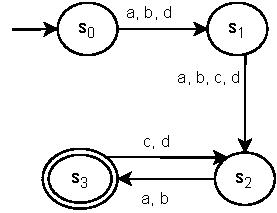
\includegraphics[height=100pt]{mintermization_automaton_m1.pdf}
        \caption{Finite automaton $M_1$ with transitions $\delta_1$.}
        \label{fig:diagram:mintermization_automaton_m1}
    \end{minipage}
    \hfill
    \begin{minipage}{0.49\linewidth}
        \centering
        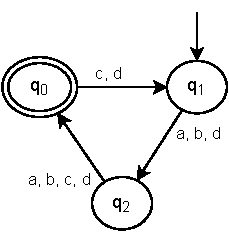
\includegraphics[height=100pt]{mintermization_automaton_m2.pdf}
        \caption{Finite automaton $M_2$ with transitions $\delta_2$.}
        \label{fig:diagram:mintermization_automaton_m2}
    \end{minipage}
    \vspace{0.5cm}
    \caption{Finite automata $M_1$ and $M_2$ used as example automata for mintermization.}
    \label{fig:diagram:mintermization_automata}
\end{figure*}

The Figure~\ref{fig:diagram:mintermization_automata_transition_sets} depicts how we could mark each transition set in our automata to be used in mintermization process. For example, a transition set $\varphi_1$ could be a set of transition symbols from state $s_0$ to $s_1$: $\varphi_i = {a, b, d}$. Similarly, we mark the remaining transition sets. Now, we can proceed to execute mintermization operations.

\begin{figure*}[ht]
    \centering
    \begin{minipage}{0.49\linewidth}
        \centering
        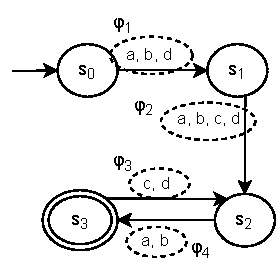
\includegraphics[height=100pt]{obrazky-figures/mintermization_automaton_m1_with_transition_sets.pdf}
        \caption{Finite automaton $M_1$ with transition sets $\varphi_i$.}
        \label{fig:diagram:mintermization_automaton_m1_with_transition_sets}
    \end{minipage}
    \hfill
    \begin{minipage}{0.49\linewidth}
        \centering
        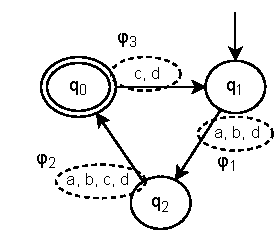
\includegraphics[height=100pt]{obrazky-figures/mintermization_automaton_m2_with_transition_sets.pdf}
        \caption{Finite automaton $M_2$ with transition sets $\varphi_i$.}
        \label{fig:diagram:mintermization_automaton_m2_with_transition_sets}
    \end{minipage}
    \vspace{0.5cm}
    \caption{Finite automata $M_1$ and $M_2$ with marked transition sets used in mintermization.}
    \label{fig:diagram:mintermization_automata_transition_sets}
\end{figure*}

If we were to compute minterms for these automata, we would proceed as follows: Starting with the whole alphabet of both automata\footnote{If the automata had non-equal alphabets, we would start with their intersection: $\Sigma = \Sigma_1 \cap \Sigma_2$} at the top of the minterm tree to be generated. Afterwards, we iterate over transition sets. For each transition set $\varphi_i$, we compute the intersection of the current minterm tree leaves with:
\begin{itemize}
    \item the current transition set $\varphi_i$ and store the result as a left node of this particular tree node,
    \item the complement of the current transition set $Q \setminus \varphi_i$ and store the result as a right tree node of this particular tree node.
\end{itemize}

If the intersection is empty, we omit creating the corresponding child node entirely. In the end, we are left with a complete minterm tree for the given set of transition sets $\Phi$ representing the specified finite automata.

The Figure~\ref{fig:diagram:mintermization_example} illustrates our mintermization process in a~diagram.

\begin{figure}[ht]
	\centering
	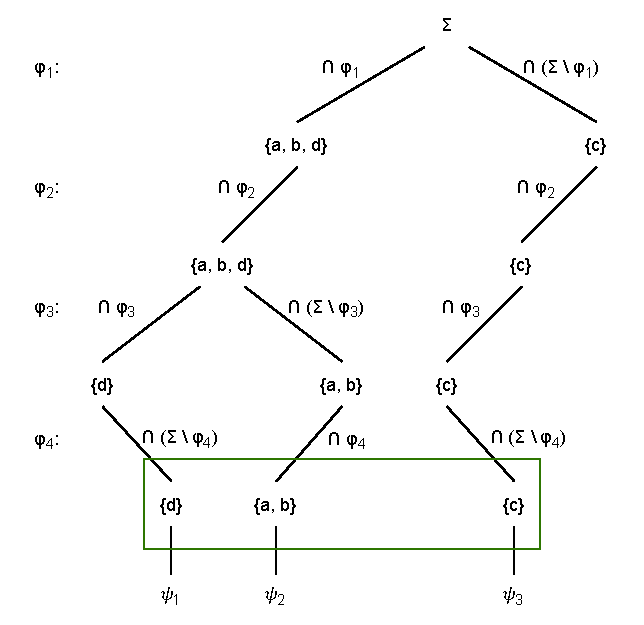
\includegraphics[width=0.7\linewidth]{mintermization_example.pdf}
	\caption{Mintermization process executed on example finite automata $M_1$ and $M_2$. We start with the whole alphabet and make our way down through all mintermization sets $\varphi_i$, where $1 \leq i \leq n$. For each mintermization set, we compute the intersection of the preceding set with the current mintermization set $\varphi_i$. The results are shown in the diagram as the nodes of the tree. When operations on all mintermization sets were executed, the leaves of the tree (indicated by the green square) represent the final minterms for the given mintermization sets $\Phi$ over the given alphabet $\Sigma$. We denote each minterm $\psi_i$, where $1 \leq i \leq |\Psi|$ where $|\Psi|$ represents the total number of generated minterms.}
	\label{fig:diagram:mintermization_example}
\end{figure}

The acquired minterms are:
$$ \Psi = Minterms(\Phi) = \{ \{d\}, \{a, b\}, \{c\} \} = \{ \psi_1, \psi_2, \psi_3 \} \text{.}$$

We can now substitute the former transition sets $\varphi_i$ for finite automata with the appropriate minterms $\psi_j, 1 \leq j \leq |\Psi|$ which were created from the specific transition sets $\varphi_i \in \Phi$ such that $\varphi_i$ is used in its direct form (not as a complement) in the process of computing $\psi_j$. The resulting automata can be seen in Figure~\ref{fig:diagram:mintermization_automata_with_minterms}.

\begin{figure*}[ht]
    \centering
    \begin{minipage}{0.49\linewidth}
        \centering
        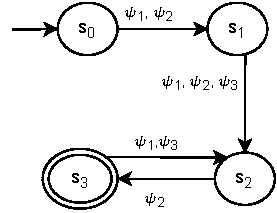
\includegraphics[height=100pt]{mintermization_automaton_m1_with_minterms.pdf}
        \caption{Finite automaton $M_1$ with transitions substituted by corresponding minterms $psi_i \in \Psi$ created from these transition sets.}
        \label{fig:diagram:mintermization_automaton_m1_with_minterms}
    \end{minipage}
    \hfill
    \begin{minipage}{0.49\linewidth}
        \centering
        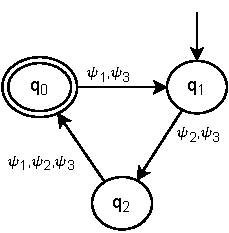
\includegraphics[height=100pt]{mintermization_automaton_m2_with_minterms.pdf}
        \caption{Finite automaton $M_2$ with transitions substituted by corresponding minterms $psi_i \in \Psi$ created from these transition sets.}
        \label{fig:diagram:mintermization_automaton_m2_with_minterms}
    \end{minipage}
    \vspace{0.5cm}
    \caption{Finite automata $M_1$ and $M_2$ with substituted transitions with minterms in the process of mintermization.}
    \label{fig:diagram:mintermization_automata_with_minterms}
\end{figure*}

Consequently, assuming the previously said, considering we have minterms over alphabet of $A$, we know that the intersection of two minterms has to be an empty set and that $\forall \psi \in \Psi: \psi \subseteq \varphi, \varphi \in \Phi$ if $\psi$ is created from $\varphi$. We make use of this knowledge further.

In the following section, we propose a method of using minterm computation with Parikh image computation optimization. We choose this approach in order to mitigate the disadvantages of Parikh image computation for finite automata, especially those with multitude of transitions between two states varying only in transition symbols, which require considerate time to compute and evaluate. This method proceeds to represent such sets of transitions between two states with a single minterm representing these transitions. We can therefore apply any previously mentioned optimization methods (or any other known optimization method) on such modified automata with minterms as their transition symbols to construct their product without the need to compute, for example, Parikh image for every single transition symbol between two states. We can now compute possibly fewer transitions with the resulting minterms instead.

% TODO: Algorithm using minterms for computation methods.


%TODO

%--------------------------------------------------------
%--------------------------------------------------------
%--------------------------------------------------------
%--------------------------------------------------------
\chapter{Experiments and Results}\label{experimentsAndResultsChapter}

The reference implementation\footnote{In the \href{https://github.com/Adda0/optimizing_automata_product_construction_and_emptiness_test}{reference implementation}, we use \href{https://github.com/Z3Prover/z3}{Z3} as an SMT solver and automata operations are handled by \href{https://github.com/Adda0/symboliclib}{for our uses modified library Symboliclib}.} of optimization, written in Python 3, as well as a complete table of all of our experiments and their results and graphs is publicly accessible on a \href{https://github.com/Adda0/optimizing_automata_product_construction_and_emptiness_test}{GitHub repository}\footnote{{\href{https://github.com/Adda0/optimizing_automata_product_construction_and_emptiness_test}{https://github.com/Adda0/optimizing\_automata\_product\_\\construction\_and\_emptiness\_test}}}. There is further explanation of the following graphs as well as additional graphs with description and in-depth analysis of performed experiments.


Test benchmarks used in our experiments were obtained from regular model checking. We have tested various different finite automata and their combinations. We have often used the same automata with their slightly changed variations to simulate real world examples of usually used automata to see how the optimized algorithm reduces the generated state space for certain types of automata with their typical qualities.

We have tested two main aspects:
\begin{itemize}
    \item First, we have tested the generated state space for emptiness test. That is, whenever we find a solution---accepting state in the intersection, the test ends, and we count the number of generated product states to this moment. If no intersection is found, we end the test when it is certain there is no accepting state and the intersection is indeed empty.
    \item Second, for the same pair of automata, we have tested the full product construction. Adding new accepting states along the way and comparing generated state spaces in the end for the full product accepting the whole intersection of original automata.
\end{itemize}

The following graphs show the results for both the emptiness test and full product construction. The graph in Figure~\ref{fig:graph:et_state_space_sizes_comp} shows the comparison of product state spaces sizes in basic product construction algorithm and our optimized algorithm considering length abstraction for emptiness test. Sorted in order of increasing product state space size generated by the basic product construction algorithm. The graph in Figure~\ref{fig:graph:fp_state_space_sizes_comp} shows the same data, only for the full product construction experiment.

\begin{figure*}[ht]
    \centering
    \begin{minipage}{0.49\linewidth}
        \centering
        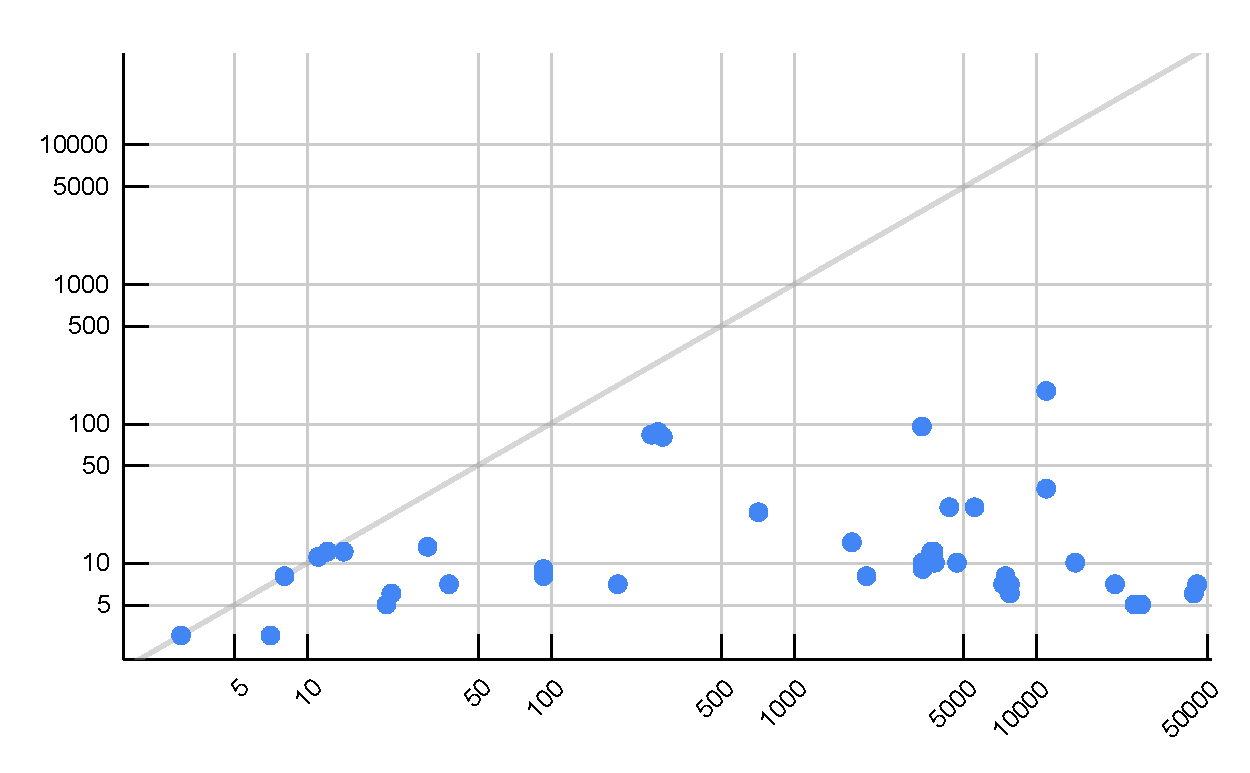
\includegraphics[width=\linewidth]{graph_scatter_et.pdf}
        \caption{Emptiness test}
        \label{fig:graph:et_state_space_sizes_comp}
    \end{minipage}
    \hfill
    \begin{minipage}{0.49\linewidth}
        \centering
        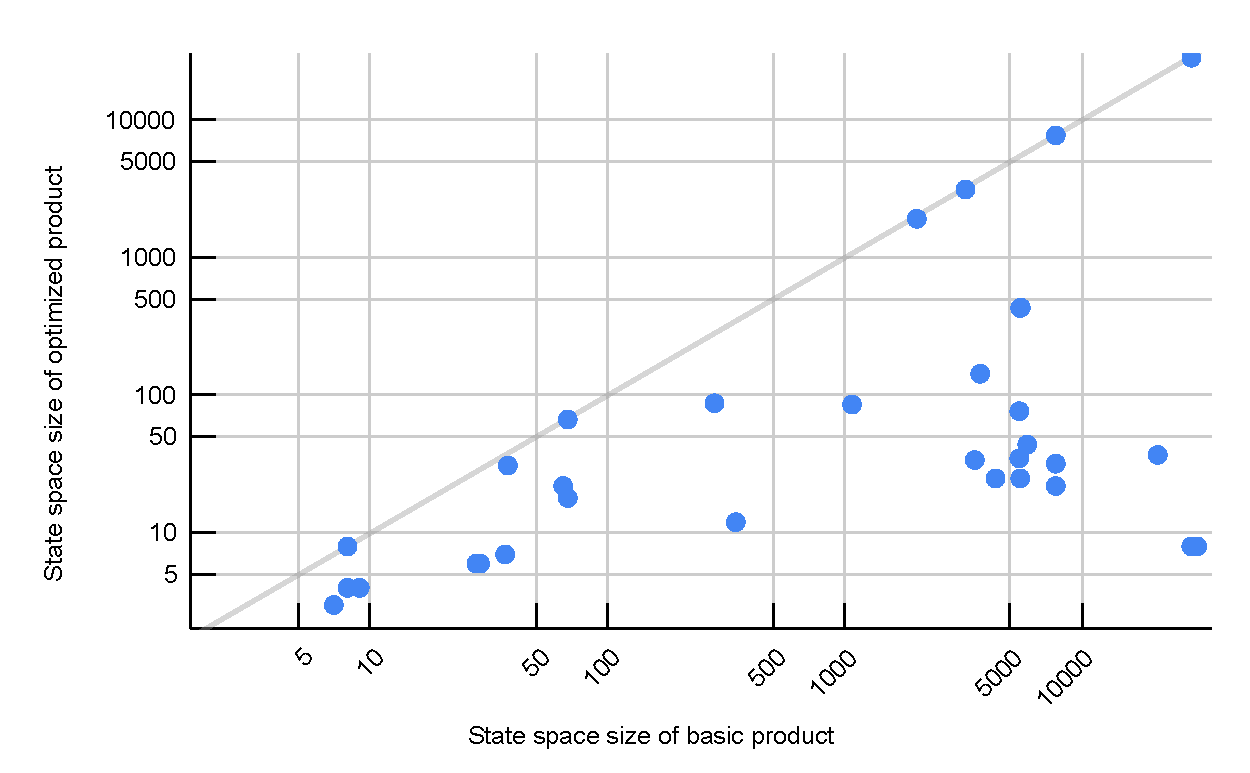
\includegraphics[width=\linewidth]{graph_scatter_fp.pdf}
        \caption{Full product construction}
        \label{fig:graph:fp_state_space_sizes_comp}
    \end{minipage}
    \vspace{0.5cm}
    \caption{Comparison of state space sizes generated by basic and optimized product construction algorithms. Both axes are in logarithmic scale, x-axis showing state space sizes of basic product, y-axis state space sizes of optimized product.}
    \label{fig:graph:product_state_space_sizes}
\end{figure*}

Where the length abstraction cannot optimize the product construction, both products have about the same state space size. These results are caused mostly by constructing products of two almost identical automata with only a few states/transitions missing/added which do not affect the accepting runs for recognized languages. There are therefore no branches which can be trimmed---most of the processed states are evaluated as \emph{satisfiable} in length abstraction satisfiability check. In full product construction results, if there are nearly no product states to trim, the generated product state space size \emph{explodes} similarly to the basic product construction algorithm---typical for automata with large numbers of transitions from every state causing large numbers of possible accepted lengths, where our algorithm can trim only a few states.

For another automata, the product generated by our algorithm is much smaller. We can see from the graphs that the larger the basic product state space size gets, the higher impact our optimization has on the product state space size. The same holds for the full product construction results. For cases where the intersection is truly empty and accepted lengths differ in both automata, our algorithm stops the process of product construction on the very first tested product state. The basic algorithm continues to create a full product.

We get the best results for automata with practically the same transitions which differ only slightly in final states or a few transitions which affects the accepting runs in the original automata. These changes cause the basic algorithm to generate the product states without realizing most (if not all) product states do not lead to an accepting state. These slight differences in automata (especially in final states) usually also change the length of accepted words. Therefore, our optimization is able to notice these differences and trim most of the product state space, if not the whole product, when no final state can be accessed and the intersection is empty.

In both graphs, we can see the aforementioned quadratic state space explosion for product is nearly not affecting our algorithm in comparison to the basic product construction algorithm. Optimized products are easier to work with and operations on such products require less computational time and memory consumption.

It is worth mentioning that we have neglected the number of generated state space for our lasso automata this whole time. We can use deterministic minimization on original automata to further optimize the generated state space for lasso automata and products. However, we do not need these lasso automata after product construction is complete. Therefore, the lasso automata do not affect how efficiently we work with the generated product. Nevertheless, the number of generated lasso states in the process of deciding the intersection emptiness test matters. For different automata, the generated state space varies. For state space sizes of lasso automata in our experiments, see \href{https://github.com/Adda0/optimizing_automata_product_construction_and_emptiness_test/tree/master/results}{the GitHub repository}\footnote{{\href{https://github.com/Adda0/optimizing_automata_product_construction_and_emptiness_test/tree/master/results}{https://github.com/Adda0/optimizing\_automata\_product\\\_construction\_and\_emptiness\_test/tree/master/results}}}.

\begin{figure*}[ht]
    \centering
    \begin{minipage}{0.49\linewidth}
        \centering
        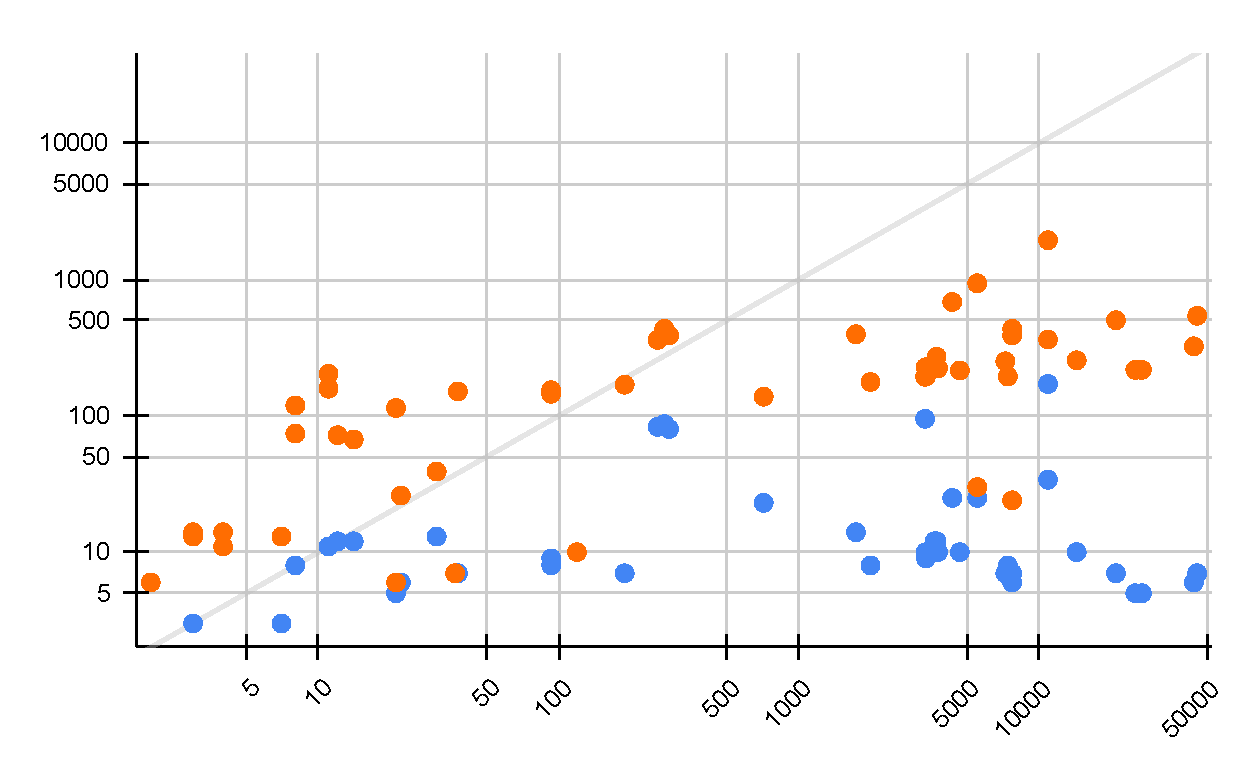
\includegraphics[width=\linewidth]{graph_scatter_combined_et.pdf}
        \caption{Emptiness test}
        \label{fig:graph:et_state_space_sizes_comp_with_lasso}
    \end{minipage}
    \hfill
    \begin{minipage}{0.49\linewidth}
        \centering
        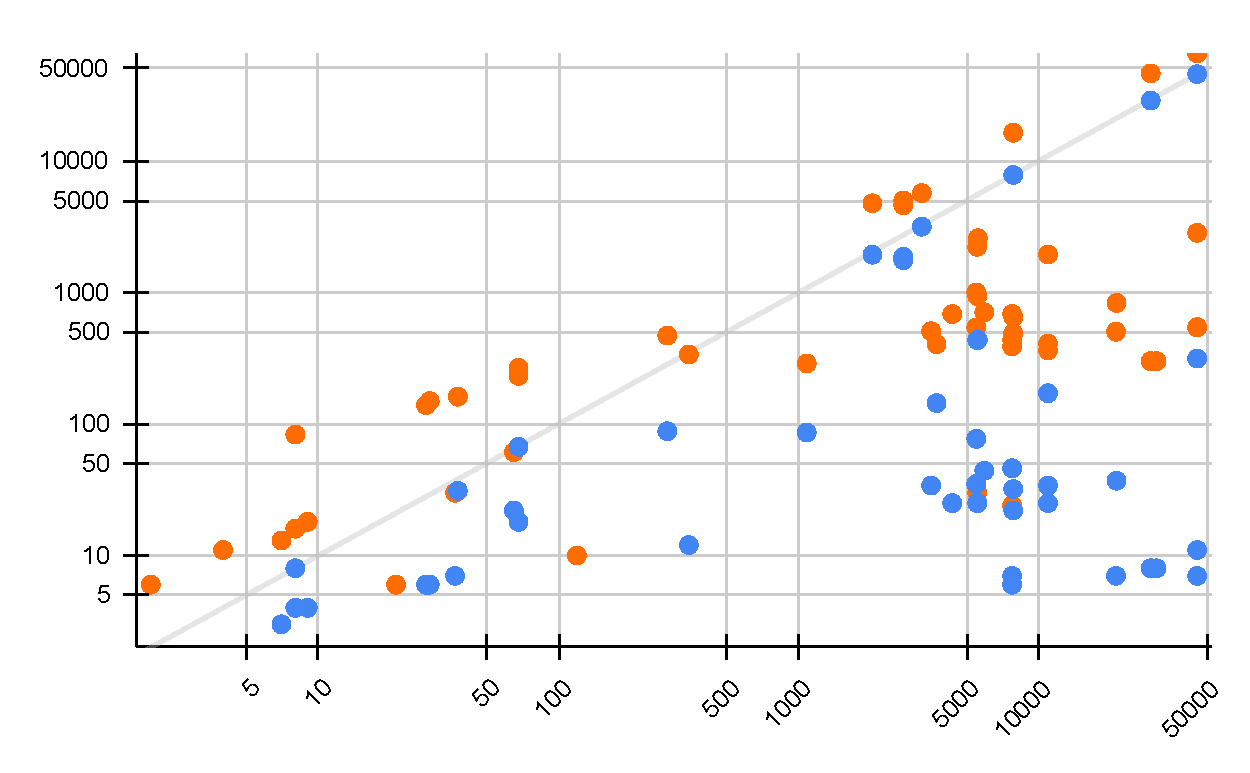
\includegraphics[width=\linewidth]{graph_scatter_combined_fp.pdf}
        \caption{Full product construction}
        \label{fig:graph:fp_state_space_sizes_comp_with_lasso}
    \end{minipage}
    \vspace{0.5cm}
    \caption{Comparison of state space sizes generated by basic and optimized product construction algorithms with sum of states generated for both the final optimized product and lasso automata states generated in the process of the product construction. Both axes are in logarithmic scale, x-axis showing state space sizes of basic product, y-axis state space sizes of optimized product (and optimized product with lasso automata states). The blue dots represent only the optimized product state space sizes (as in Figure~\ref{fig:graph:product_state_space_sizes}), the orange dots the sum of optimized product state space sizes and the generated lasso states.}
    \label{fig:graph:product_state_space_sizes_with_lasso}
\end{figure*}

As we can see in Figure~\ref{fig:graph:product_state_space_sizes_with_lasso}, even when counting with lasso automata product state space sizes, the total number of generated states in the whole process of the product construction is usually lower than the basic product state space size. The larger the automata are, the better results we get. It is understandable, that for smaller original automata, whose intersection is computed, the expense of generating lasso automata is significant in comparison with the generated product state space sizes. The larger the original automata get, the lesser the expense of the number of lasso automata states is in comparison with the basic product state space.

\begin{figure*}[ht]
    \centering
    \begin{minipage}{0.49\linewidth}
        \centering
        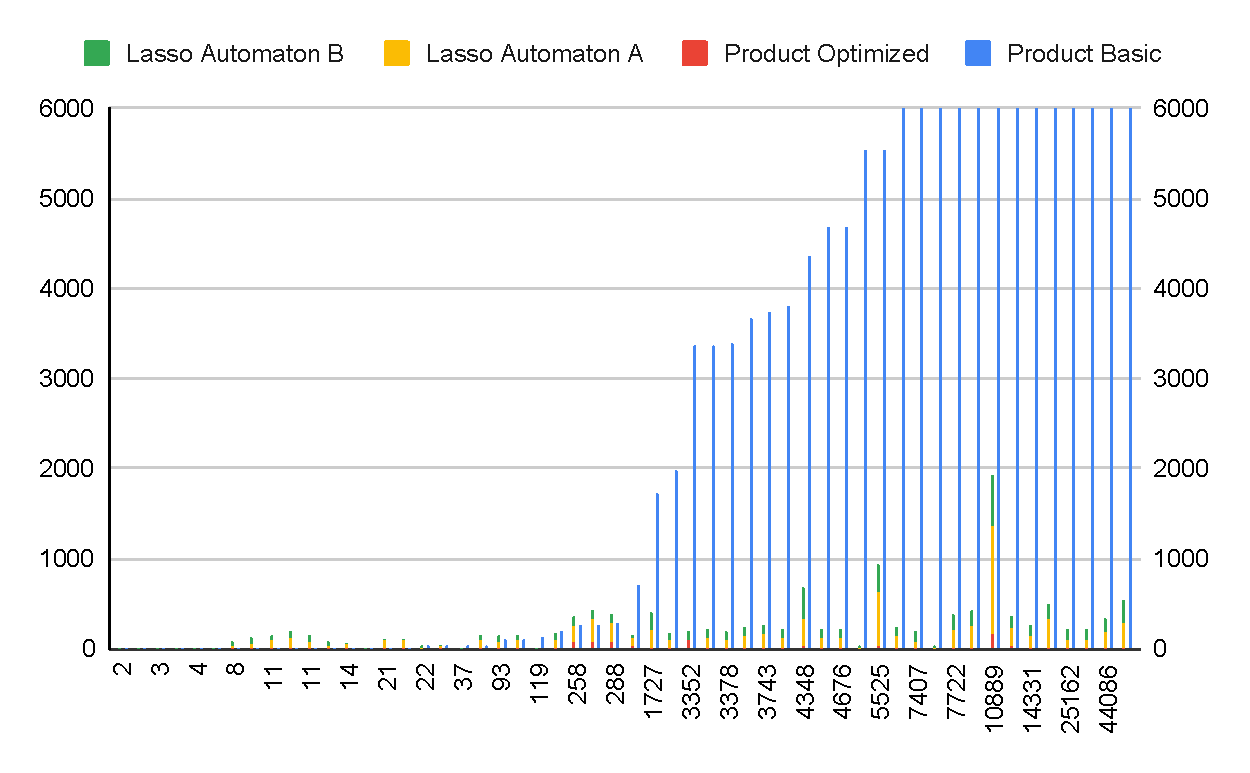
\includegraphics[width=\linewidth]{graph_stacked_et.pdf}
        \caption{Emptiness test}
        \label{fig:graph:stacked_et_state_space_sizes_comp_with_lasso}
    \end{minipage}
    \hfill
    \begin{minipage}{0.49\linewidth}
        \centering
        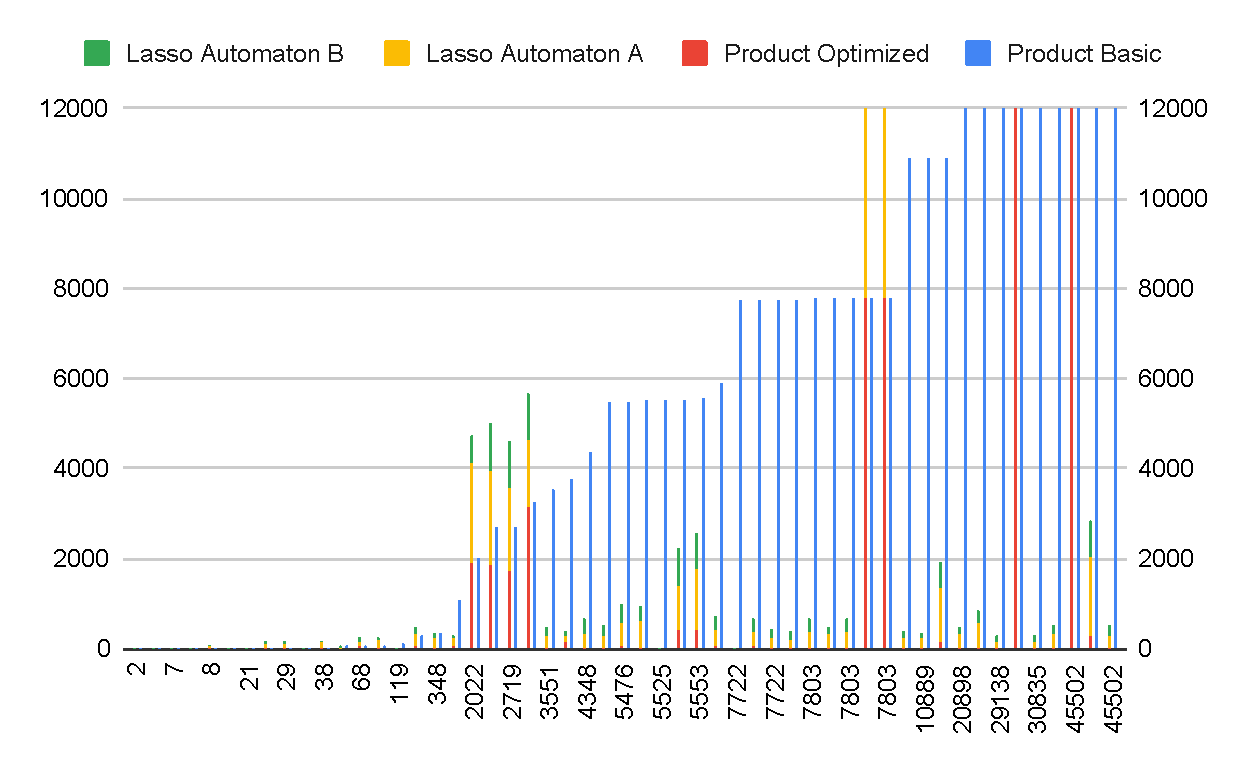
\includegraphics[width=\linewidth]{graph_stacked_fp.pdf}
        \caption{Full product construction}
        \label{fig:graph:stacked_fp_state_space_sizes_comp_with_lasso}
    \end{minipage}
    \vspace{0.5cm}
    \caption{Stacked comparison of state space sizes generated by basic and optimized product construction algorithms with sum of states generated for both the final optimized product and lasso automata states generated in the process of the product construction. Both axes are in logarithmic scale, x-axis showing state space sizes of basic product (ordered in ascending order), y-axis state space sizes of depicted experiments---because of huge differences in sizes of basic product and optimized product with lasso automata, the largest shown values are set to 6000 and 12000, respectively. Each two columns show a single experiment with our optimized solution as the left (green, red and orange) column---as a sum of all generated states (of optimized product (green) and both lasso automata (red and orange), and the right blue column as the basic product state space size).}
    \label{fig:graph:stacked_product_state_space_sizes_with_lasso}
\end{figure*}

Out of all experiments, one weakness of our algorithm is clear---the more final states the original automata have, the more difficult it is to optimize the full product construction using length abstraction. This is caused by the fact that every final state increases the number of accepted different lengths per automaton. Therefore, with automata where out of hundreds or thousands of states nearly every state is a final state too, our optimization algorithm has to consider multiple possible lengths and cannot easily determine which branches will not be accepted by the product automaton.

%--------------------------------------------------------
%--------------------------------------------------------
%--------------------------------------------------------
%--------------------------------------------------------
\chapter{Conclusion}

The most demanding parts of the intersection computation is the generation of product states and transitions of the product automaton. We tried to reduce the size of the generated state space by omitting the states which cannot lead to any accepting state---that is, omitting the \textit{branches} which do not lead to any accepting state---by computing the emptiness test of these states using length abstraction over the original automata using lasso automata.

According to our experiments, product state space is minimized especially for intersections with huge non-terminating branches or for intersections of automata accepting different lengths of words recognized by the automata languages. Further, for automata with long lines and similar automata varying only slightly from each other. Experiments show our algorithm generates smaller product state spaces for both emptiness test and full product construction, which are two most usually used operations on automata intersection. And because length abstraction considers over-approximation of possible products, our algorithm is safe to use for any uses resolving automata intersection.

We have not encountered similar approaches to product construction optimization using length or other abstraction to compare our results with. It might be worth investing into combining our orthogonal approach with other existing algorithm to see how the generated product state space is affected. We are talking about abstraction techniques such as CEGAR \cite{DBLP:conf/cav/ClarkeGJLV00} and predicate abstraction \cite{DBLP:conf/cav/ColonU98, DBLP:conf/cav/GrafS97}, IMPACT \cite{DBLP:conf/cav/McMillan06}, possibly IC3/PDR \cite{DBLP:conf/sat/HoderB12, DBLP:conf/fmcad/BradleyM07}. All the above techniques have proven efficient in hardware or software verification, and they can be applied in automata too. First attempts to use these techniques in finite automata problem-solving are based on IC3 \cite{DBLP:journals/pacmpl/HolikJLRV18, DBLP:conf/cav/WangTLYJ16, DBLP:journals/corr/abs-1708-09073} and on the interpolation-based approach of McMillan \cite{DBLP:conf/tacas/AmlaM07, DBLP:conf/tacas/GangeNSSS13}.

We can also compute Parikh images using Parikh theorem \cite{Kozen1977} instead of just lengths of recognized words. Parikh images give us additional information about every product state. This allows more precise estimation of possible accepted words by both automata and deciding the emptiness test of their intersection more effectively. Computation of Parikh image is time-consuming, but might further minimize the product construction state space.

